\documentclass[a4paper,titlepage,oneside,12pt]{amsart} %amsart
\usepackage{graphicx}
\usepackage{hyperref}
%\usepackage{geometry} % see geometry.pdf on how to lay out the page. There's lots.
\usepackage[margin=1.3in]{geometry}
\geometry{a4paper} % or letter or a5paper or ... etc
% \geometry{landscape} % rotated page geometry
\usepackage{ifthen}

% See the ``Article customise'' template for come common customisations
\usepackage[usenames,dvipsnames]{color}

\usepackage[table]{xcolor}

\definecolor{lightgray}{RGB}{245, 245, 245}
\definecolor{bkblue}{RGB}{18, 47, 76}
\definecolor{bklightblue}{RGB}{102, 131, 158}
\definecolor{mygreen}{rgb}{0,0.6,0}
\definecolor{orange}{RGB}{255,153,0}

\usepackage{opensans}
\usepackage{setspace}
\usepackage{booktabs} \newcommand{\ra}[1]{\renewcommand{\arraystretch}{#1}}

\usepackage{color}

% show todos
\newcommand{\todo}[1]{\colorbox{yellow}{#1}}
% ignore todos
% \newcommand{\todo}[1]{}

\newcommand{\toread}[1]{{\color{bklightblue} #1}}

\usepackage{listings}
\lstset{ %
float,
language=C,                % choose the language of the code
basicstyle=\footnotesize,       % the size of the fonts that are used for the code
%numbers=left,                   % where to put the line-numbers
%numberstyle=\footnotesize,      % the size of the fonts that are used for the line-numbers
%stepnumber=1,                   % the step between two line-numbers. If it is 1 each line will be numbered
%numbersep=5pt,                  % how far the line-numbers are from the code
backgroundcolor=\color{lightgray},  % choose the background color. You must add \usepackage{color}
showspaces=false,               % show spaces adding particular underscores
showstringspaces=false,         % underline spaces within strings
showtabs=false,                 % show tabs within strings adding particular underscores
frame=single,           % adds a frame around the code
framerule=0.2pt,
tabsize=2,          % sets default tabsize to 2 spaces
captionpos=b,           % sets the caption-position to bottom
breaklines=true,        % sets automatic line breaking
breakatwhitespace=false,    % sets if automatic breaks should only happen at whitespace
escapeinside={\%*}{*)},          % if you want to add a comment within your code
belowcaptionskip=5em,
belowskip=1em,
aboveskip=1.8em,
commentstyle=\itshape\color{mygreen},
keywordstyle=\bfseries\color{black},
identifierstyle=\color{black},
stringstyle=\color{blue},
morekeywords={*, timer_source_t, data_source_t, uint32_t, uint16_t, uint8_t, RUN_LOOP_TYPE, le_command_status_t, gatt_client_t,
 							le_characteristic_t, le_service_t, le_characteristic_descriptor_t, service_record_item_t, bd_addr_t, btstack_packet_handler_t,
							hci_cmd_t, bt_control_t, remote_device_db_t, link_key_t, device_name_t, hci_transport_t, hci_uart_config_t, sdp_query_event_t,
							sdp_query_complete_event_t, sdp_query_rfcomm_service_event_t, sdp_parser_event_t, sdp_parser_event_type_t,
							sdp_parser_attribute_value_event_t, sdp_parser_complete_event_t, advertising_report_t, gc_state_t, le_service_event_t,
							le_characteristic_event_t}
}

% Bluetopia & TI MSP430 + Stellaris
% http://processors.wiki.ti.com/index.php/CC256x_Bluetopia_Stack#Demos

% Setup MSP430+PAN1315
% 
\newcommand{\versionNr}{1.3}
\newcommand{\authorMila}{Dr. sc. Milanka Ringwald}
\newcommand{\authorMatthias}{Dr. sc. Matthias Ringwald}
\newcommand{\bkContact}{\href{contact@bluekitchen-gmbh.com}{contact@bluekitchen-gmbh.com}}
\newcommand{\barWidth}{0.3cm}
\newcommand{\urlfoot}[2]{\href{#1}{{\color{blue} #2}}\footnote{#1}}

\makeatletter
\renewcommand{\maketitle}{
  \begin{titlepage}
    \fosfamily
    \begin{center}
    \begin{minipage}[b]{\textwidth}
        \begin{minipage}[b]{.1\textwidth}
            \color{bkblue}\rule{\barWidth{}}{22cm}
        \end{minipage}
        \hfill\begin{minipage}[b]{.8\textwidth}\begin{flushright}
            {\color{bkblue}VERSION \versionNr{} \\
            \today \\}
            \vspace*{7.5cm}
            \hfill
\includegraphics[width=0.85\textwidth]{picts/bklogo.pdf}
            \vspace*{1.5cm}
            \begin{spacing}{2} 
                {\huge \color{bkblue} \@title} \\ 
                {\Large \color{bklightblue} Including Quickstart Guide}   
            \end{spacing} 
            \vspace*{1.5cm}
            {\color{bkblue}\large \authorMila \\
            \large \authorMatthias \\
            \large \bkContact\\ }
        \end{flushright}\end{minipage}
        \vfill
        \begin{minipage}[b]{\textwidth}
            \color{bklightblue}\rule{\barWidth{}}{\barWidth{}}
        \end{minipage}
    \end{minipage}

    
    \end{center}
  \end{titlepage}
}
\makeatother

\title[BTstack Manual] {BTstack Manual} 
\author{Copyright \copyright 2012-2015 BlueKitchen GmbH}

%%% BEGIN DOCUMENT

\newcommand{\UserGuide}{\urlfoot{http://processors.wiki.ti.com/index.php/PAN1315EMK\_User\_Guide\#RF3\_Connector}{User Guide}{}}
\newcommand{\MSPGCCWiki}{\urlfoot{http://sourceforge.net/apps/mediawiki/mspgcc/index.php?title=MSPGCC\_Wiki}{MSPGCC Wiki}}
\newcommand{\GNUMake}{\urlfoot{http://gnuwin32.sourceforge.net/packages/make.htm}{GNU Make}}
\newcommand{\Python}{\urlfoot{http://www.python.org/getit/}{Python}}
\newcommand{\mspgcc}{\urlfoot{http://sourceforge.net/projects/mspgcc/files/Windows/mingw32/}{mspgcc}}
\newcommand{\BTSfile}{\urlfoot{http://processors.wiki.ti.com/index.php/CC256x\_Downloads}{BTS file}}
\newcommand{\MSPFlasher}{\urlfoot{http://processors.wiki.ti.com/index.php/MSP430\_Flasher\_-\_Command\_Line\_Programmer}{MSP430Flasher}}
\newcommand{\MSPDebug}{\urlfoot{http://mspdebug.sourceforge.net/}{MSPDebug}}
\newcommand{\BtstackGithub}{\urlfoot{https://github.com/bluekitchen/btstack/archive/master.zip}{BTstack's page}}
\newcommand{\gccarm}{\urlfoot{https://launchpad.net/gcc-arm-embedded}{arm-gcc}}
\newcommand{\OpenOCD}{\urlfoot{http://openocd.org}{OpenOCD}}
\newcommand{\mplabxc}{\urlfoot{http://www.microchip.com/pagehandler/en\_us/devtools/mplabxc/}{MPLAB XC}}
\newcommand{\PICkit}{\urlfoot{http://www.microchip.com/DevelopmentTools/ProductDetails.aspx?PartNO=pg164130}{PICkit 3}}

%level -1: part, 0: chapter, 1: section, etc.
\setcounter{tocdepth}{3}

\begin{document}

\maketitle

\tableofcontents
\pagebreak


Thanks for checking out BTstack! In this manual, we first provide the usual 'quick starter guide' before highlighting BTstack's main design choices and going into more details with a few examples. Finally, we outline the basic steps when integrating BTstack into existing single-threaded or even multi-threaded environments. The Revision History is shown in the Appendix \ref{appendix:revision_history} on page \pageref{appendix:revision_history}.

\section{Quick Start}

\subsection{General Tools}
On Unix-based systems, git, make, and Python are usually installed. If not, use the system's packet manager to install them. 

On Windows, you need to install and configure mspgcc, GNU Make, Python, and optionally git manually:
 \begin{itemize}
 \item \GNUMake{} for Windows: Add its bin folder to the Windows Path in Environment Variables. The bin folder is where make.exe resides, and it's usually located in \path{C:\Program Files\GnuWin32\bin}. 
 \item \Python{} for Windows: Add Python installation folder to the Windows Path in Environment Variables.
 \end{itemize}

Adding paths to the Windows Path variable:
\begin{itemize} \label{sec:windowsPath}
   \item Go to: Control Panel$\rightarrow$System$\rightarrow$Advanced tab$\rightarrow$Environment Variables.
   \item The top part contains a list of User variables. 
   \item Click on the Path variable and then click edit.
   \item Go to the end of the line, then append the path to the list., for example, \path{C:\mspgcc\bin} for mspgcc.
   \item Ensure that there is a semicolon before and after \path{C:\mspgcc\bin}. 
\end{itemize}

\subsection{Getting BTstack from GitHub}

Use git to clone the latest version:
	\begin{lstlisting}
 		git clone https://github.com/bluekitchen/btstack.git
	\end{lstlisting}
Alternatively, you can download it as a ZIP archive from \BtstackGithub{}on GitHub.

\subsection{Compiling the examples and loading firmware}
This step is platform specific. To compile and run the examples, you need to download and install the platform specific toolchain and a flash tool. For TI's CC256x chipsets, you also need the correct init script, or "Service Pack" in TI nomenclature. Assuming that these are provided, go to \path{btstack/platforms/$PLATFORM$} folder in command prompt and run make. If all the paths are correct, it will generate several firmware files. These firmware files can be loaded onto the device using platform specific flash programmer. For the PIC32-Harmony platform, a project file for the MPLAB X IDE is provided, too.

\begin{table*}\centering
\caption{Overview of platform specific toolchains, programmers, and used chipsets.}

\resizebox{\textwidth}{!}{\begin{minipage}{\textwidth}
\rowcolors{1}{lightgray}{white}

\begin{tabular}{p{4cm}p{2cm}p{3cm}p{4cm} }
\toprule
\hiderowcolors Platform & Chipset & Toolchain & Programmer\\ \showrowcolors
\midrule
ez430-rf2560, msp-exp430f5438,  msp430f5229lp & CC256x & \mspgcc{} &\MSPFlasher{},  \MSPDebug{} \\           
stm32-f103rb-nucleo     & CC256x   & \gccarm{}    & \OpenOCD{} \\      
pic32-harmony               & CSR8811 & \mplabxc{} & \PICkit{} \\ \hiderowcolors
\bottomrule
 \label{table:platformCompiler}
 \end{tabular}
 
 \end{minipage} }
\end{table*}

\subsection{Run the Example}

As a first test, we recommend the SPP Counter example (see Section \ref{section:sppcounter}). During the startup, for TI chipsets, the init script is transferred, and the Bluetooth stack brought up. After that, the development board is discoverable as "BTstack SPP Counter" and provides a single virtual serial port. When you connect to it, you'll receive a counter value as text every second.

% The SPP Counter doesn't use the display to keep the memory footprint small.
%  The HID demo has a fancier user interface - it uses a display to show the discovery process and connection establishment with a Bluetooth keyboard, as well as the text as you type.
 
\subsection{Platform specifics}
 
% !TEX root = btstack_gettingstarted.tex

In the following, we provide more information on specific platform setups, toolchains, programmers, and init scripts.
\subsubsection{libusb}
$ $

The quickest way to try BTstack is on a Linux or OS X system with an additional USB Bluetooth module. The Makefile in \path{platforms/libusb} requires \pkgconfig{} and \libusb{}-1.0 or higher to be installed. 

On Linux, it's usually necessary to run the examples as root as the kernel needs to detach from the USB module.

On OS X, it's necessary to tell the OS to only use the internal Bluetooth. For this, execute:
\begin{lstlisting}
sudo nvram bluetoothHostControllerSwitchBehavior=never
\end{lstlisting}

It's also possible to run the examples on Win32 systems. For this:
\begin{itemize}
\item Install \MSYS{} and \MINGW{} using the MINGW installer
\item Compile and install libusb-1.0.19 to /usr/local/ in msys command shell
\item Setup a USB Bluetooth dongle for use with libusb-1.0:
	\begin{itemize}
	\item Start \Zadig{}
	\item Select Options $\rightarrow$ "List all devices"
	\item Select USB Bluetooth dongle in the big pull down list
	\item Select WinUSB (libusb) in the right pull pull down list
	\item Select "Replace Driver"
	\end{itemize}
\end{itemize}
Now, you can run the examples from the $msys$ shell the same way as on Linux/OS X.

\subsubsection{Texas Instruments MSP430-based boards}
$ $

\textbf{Compiler Setup.} The MSP430 port of BTstack is developed using the Long Term Support (LTS) version of mspgcc. General information about it and installation instructions are provided on the \MSPGCCWiki{}. On Windows, you need to download and extract \mspgcc{} to \path{C:\mspgcc}. Add \path{C:\mspgcc\bin} folder to the Windows Path in Environment variable as explained in Section \ref{sec:windowsPath}.

\textbf{Loading Firmware.} To load firmware files onto the MSP430 MCU for the MSP-EXP430F5438 Experimeneter board, you need a programmer like the MSP430 MSP-FET430UIF debugger or something similar. The eZ430-RF2560 and MSP430F5529LP contain a basic debugger. Now, you can use one of following software tools:

 \begin{itemize}
 \item  \MSPFlasher{} (windows-only):
 	\begin{itemize}
 	   \item Use the following command, where you need to replace the \path{BINARY_FILE_NAME.hex} with the name of your application:
	\end{itemize} 
\end{itemize}
	
	   \begin{lstlisting}
 		MSP430Flasher.exe -n MSP430F5438A -w "BINARY_FILE_NAME.hex" -v -g -z [VCC]
	   \end{lstlisting}

 \begin{itemize}
	
	\item \MSPDebug{}: An example session with the MSP-FET430UIF connected on OS X is given in following listing:
\end{itemize}

\begin{lstlisting}
mspdebug -j -d /dev/tty.FET430UIFfd130 uif
... 
prog blink.hex
run
\end{lstlisting}

\subsubsection{Texas Instruments CC256x-based chipsets}
$ $

 \textbf{CC256x Init Scripts.} In order to use the CC256x chipset on the PAN13xx modules and others, an initialization script must be obtained. Due to licensing restrictions, this initialization script must be obtained separately as follows:
\begin{itemize}
\item Download the \BTSfile{} for your CC256x-based module.
\item Copy the included .bts file into \path{btstack/chipset-cc256x}
\item In \path{chipset-cc256x}, run the Python script: $./convert\_bts\_init\_scripts.py$
\end{itemize}

The common code for all CC256x chipsets is provided by $bt\_control\_cc256x.c$. During the setup, $bt\_control\_cc256x\_instance$ function is used to get  a $bt\_control\_t$ instance and passed to $hci\_init$ function. 

 \textbf{Note:} Depending on the CC256x-based module you're using, you'll need to update the reference \path{bluetooth_init_cc256...} in the Makefile to match the downloaded file.

 \textbf{Update:} For the latest revision of the CC256x chipsets, the CC2560B and CC2564B, TI decided to split the init script into a main part and the BLE part. The conversion script has been updated to detect $bluetooth\_init\_cc256x\_1.2.bts$ and adds $BLE\_init\_cc256x\_1.2.bts$ if present and merges them into a single .c file.

\subsubsection{MSP-EXP430F5438 + CC256x Platform}
\label{platform:msp430}
$ $

\textbf{Hardware Setup.} We assume that a PAN1315, PAN1317, or PAN1323 module is plugged into RF1 and RF2 of the MSP-EXP430F5438 board and the "RF3 Adapter board" is used or at least simulated. See \UserGuide{}. 

\subsubsection{STM32F103RB Nucleo + CC256x Platform}
$ $

To try BTstack on this platform, you'll need a simple adaptor board. For details, please read the documentation in \path{platforms/stm32-f103rb-nucleo/README.md}.

\subsubsection{PIC32 Bluetooth Audio Development Kit}
$ $

The PIC32 Bluetooth Audio Development Kit comes with the CSR8811-based BTM805 Bluetooth module. In the port, the UART on the DAC daughter board was used for the debug output. Please remove the DAC board and connect a 3.3V USB-2-UART converter to GND and TX to get the debug output.

In \path{platforms/pic32-harmony}, a project file for the MPLAB X IDE is provided as well as a regular Makefile. Both assume that the MPLAB XC32 compiler is installed. The project is set to use -Os optimization which will cause warnings if you only have the Free version. It will still compile a working example. For this platform, we only provide the SPP and LE Counter example directly. Other examples can be run by replacing the spp\_and\_le\_counter.c file with one of the other example files.




\section{BTstack Architecture}

As well as any other communication stack, BTstack is a collection of state machines that interact with each other. There is one or more state machines for each protocol and service that it implements. The rest of the architecture follows these fundamental design guidelines:

\begin{itemize}
\item \emph{Single threaded design} - BTstack does not use or require multi-threading to handle data sources and timers. Instead, it uses a single run loop.
\item \emph{No blocking anywhere} - If Bluetooth processing is required, its result will be delivered as an event via registered packet handlers.
\item \emph{No artificially limited buffers/pools} - Incoming and outgoing data packets are not queued.
\item \emph{Statically bounded memory (optionally)} - The number of maximum connections/channels/services can be configured.
\end{itemize}

\begin{figure}[htbp] %  figure placement: here, top, bottom, or page
   \centering
   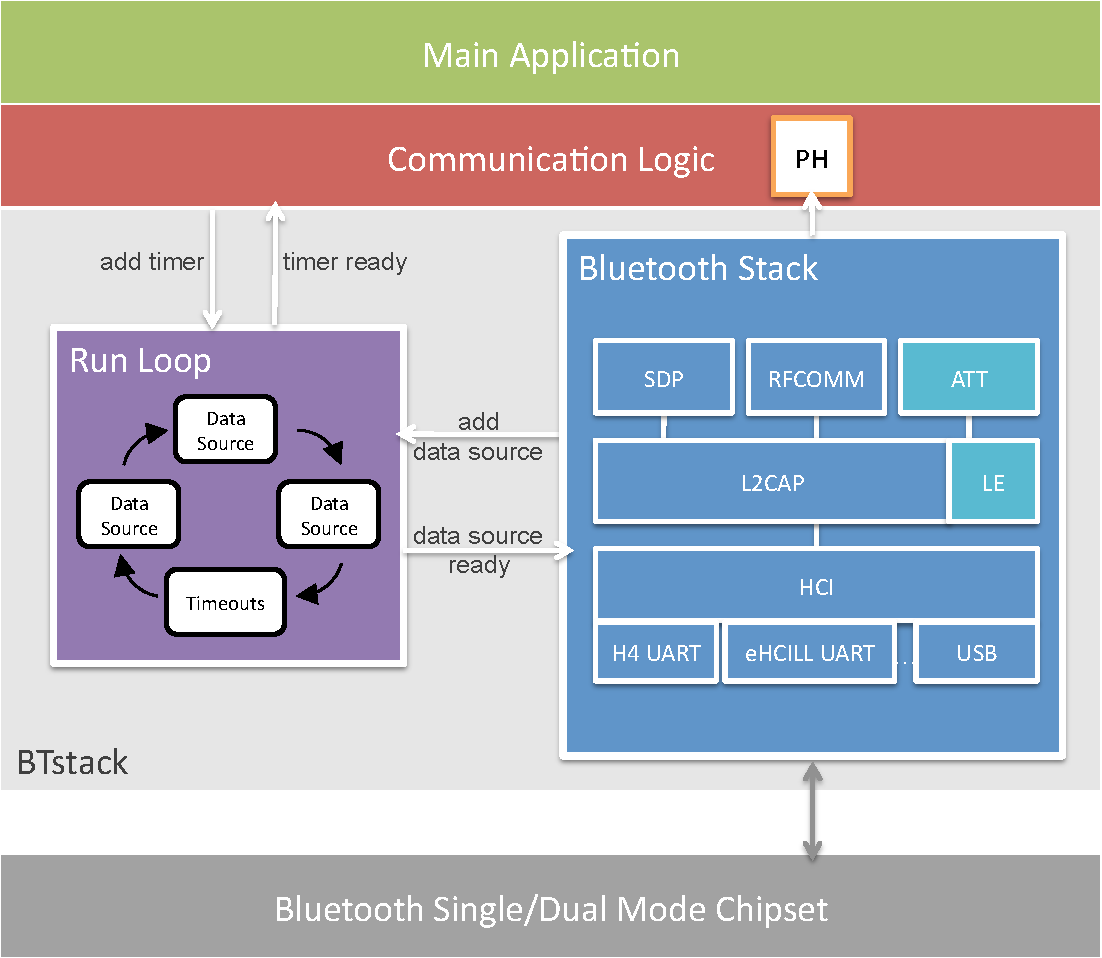
\includegraphics[width=\textwidth]{picts/btstack-architecture.pdf} 
   \caption{BTstack-based single-threaded application. The Main Application contains the application logic, e.g., reading a sensor value and providing it via the Communication Logic as a SPP Server.
    The Communication Logic is often modeled as a finite state machine with events and data coming from either the Main Application or from BTstack via registered  packet handlers (PH).   
    BTstack's Run Loop is responsible for providing timers and processing incoming data.
}
    
   \label{fig:BTstackArchitecture}
\end{figure}

Figure \ref{fig:BTstackArchitecture} shows the general architecture of a BTstack-based application that includes the BTstack run loop.

\subsection{Single threaded design}
BTstack does not use or require multi-threading. It uses a single run loop to handle data sources and timers. Data sources represent communication interfaces like an UART or an USB driver. 
Timers are used by BTstack to implement various Bluetooth-related timeouts. For example, to disconnect a Bluetooth baseband channel without an active L2CAP channel after 20 seconds. They can also be used to handle periodic events. During a run loop cycle, the callback functions of all registered data sources are called. Then, the callback functions of timers that are ready are executed. 

For adapting BTstack to multi-threaded environments, see Section \ref{section:multithreading}.


\subsection{No blocking anywhere}

Bluetooth logic is event-driven. Therefore, all BTstack functions are non-blocking, i.e., all functions that cannot return immediately implement an asynchronous pattern. If the arguments of a function are valid, the necessary commands are sent to the Bluetooth chipset and the function returns with a success  value. The actual result is delivered later as an asynchronous event via registered packet handlers. 

If a Bluetooth event triggers longer processing by the application, the processing should be split into smaller chunks. The packet handler could then schedule a timer that manages the sequential execution of the chunks.

\subsection{No artificially limited buffers/pools}
Incoming and outgoing data packets are not queued. BTstack delivers an incoming data packet to the application before it receives the next one from the Bluetooth chipset. Therefore, it relies on the link layer of the Bluetooth chipset to slow down the remote sender when needed. 

Similarly, the application has to adapt its packet generation to the remote receiver for outgoing data. 
L2CAP relies on ACL flow control between sender and receiver. If there are no free ACL buffers in the Bluetooth module, the application cannot send.  For RFCOMM, the mandatory credit-based flow-control limits the data sending rate additionally. The application can only send an RFCOMM packet if it has RFCOMM credits.

\subsection{Statically bounded memory}
BTstack has to keep track of services and active connections on the various protocol layers. The number of maximum connections/channels/services can be configured. In addition, the non-persistent database for remote device names and link keys needs memory and can be be configured, too. These numbers determine the amount of static memory allocation.


\section{How to use BTstack}
BTstack implements a set of basic Bluetooth protocols. To make use of these to connect to other devices or to provide own services, BTstack has to be properly configured during application startup. 

In the following, we provide an overview of the memory management, the run loop, and services that are necessary to setup BTstack. From the point when the run loop is executed, the application runs as a finite state machine, which processes events received from BTstack. BTstack groups events logically and provides them over packet handlers, of which an overview is provided here. Finally, we describe the RFCOMM credit-based flow-control, which may be necessary for resource-constraint devices. Complete examples for the MSP430 platforms will be presented in Chapter \ref{examples}. 

\subsection{Memory configuration}
\label{section:memory_configuration}

The structs for services, active connections and remote devices can be allocated in two different manners: 
        \begin{itemize}
        \item statically from an individual memory pool, whose maximal number of elements  is defined in the config file. To initialize the static pools, you need to call \emph{btstack\_memory\_init} function. An example of memory configuration for a single SPP service with a minimal L2CAP MTU is shown in Listing \ref{memoryConfigurationSPP}.
        \item dynamically using the \emph{malloc/free} functions, if HAVE\_MALLOC is defined in config file. 
        \end{itemize}

If both HAVE\_MALLOC and  maximal size of a pool are defined in the config file, the statical allocation will take precedence. In case that both are omitted, an error will be raised.

The memory is set up by calling \emph{btstack\_memory\_init} function:
\begin{lstlisting}
btstack_memory_init();
\end{lstlisting}


\subsection{Run loop}
\label{section:run_loop}

BTstack uses a run loop to handle incoming data and to schedule work. The run loop handles events from two different types of sources: data sources and timers. Data sources represent communication interfaces like an UART or an USB driver. Timers are used by BTstack to implement various Bluetooth-related timeouts. They can also be used to handle periodic events. 

Data sources and timers are represented by the \emph{data\_source\_t} and \emph{timer\_source\_t} structs respectively. Each of these structs contain a linked list node and a pointer to a callback function. All active timers and data sources are kept in link lists. While the list of data sources is unsorted, the timers are sorted by expiration timeout for efficient processing.

The complete run loop cycle looks like this: first, the callback function of all registered data sources are called in a round robin way. Then, the callback functions of timers that are ready are executed. Finally, it will be checked if another run loop iteration has been requested by an interrupt handler. If not, the run loop will put the MCU into sleep mode.

Incoming data over the UART, USB, or timer ticks will generate an interrupt and wake up the microcontroller. In order to avoid the situation where a data source becomes ready just before the run loop enters sleep mode, an interrupt-driven data source has to call the \emph{embedded\_trigger} function. The call to \emph{embedded\_trigger} sets an internal flag that is checked in the critical section just before entering sleep mode. 

Timers are single shot: a timer will be removed from the timer list before its event handler callback is executed. If you need a periodic timer, you can re-register the same timer source in the callback function, as shown in Listing \ref{PeriodicTimerHandler}. Note that BTstack expects to get called periodically to keep its time, see Section \ref{section:tickAbstraction} for more on the tick hardware abstraction. 

The Run loop API is provided in Appendix \ref{appendix:api_run_loop}. To enable the use of timers, make sure that you defined HAVE\_TICK in the config file.

In your code, you'll have to configure the run loop before you start it as shown in Listing \ref{RunLoopExecution}. The application can register data sources as well as timers, e.g., periodical sampling of sensors, or communication over the UART.

The run loop is set up by calling \emph{run\_loop\_init} function for embedded systems:
\begin{lstlisting}
run_loop_init(RUN_LOOP_EMBEDDED);
\end{lstlisting}


\begin{lstlisting}[float, caption=Periodic counter, label=PeriodicTimerHandler]
#define TIMER_PERIOD_MS 1000
timer_source_t periodic_timer;

void register_timer(timer_source_t *timer, uint16_t period){
    run_loop_set_timer(timer, period);
    run_loop_add_timer(timer);
}

void timer_handler(timer_source_t *ts){
    // do something,
    ... e.g., increase counter,
    
    // then re-register timer
    register_timer(ts, TIMER_PERIOD_MS);
} 

void timer_setup(){
    // set one-shot timer
    run_loop_set_timer_handler(&periodic_timer, &timer_handler);
    register_timer(&periodic_timer, TIMER_PERIOD_MS);
}
\end{lstlisting}

\subsection{BTstack initialization}
\label{section:btstack_initialization}
To initialize BTstack you need to initialize the memory and the run loop as explained in Sections \ref{section:memory_configuration} and \ref{section:run_loop} respectively, then setup HCI and all needed higher level protocols.

The HCI initialization has to adapt BTstack to the used platform and requires four arguments. These are:
\begin{itemize}
\item \emph{Bluetooth hardware control}: The Bluetooth hardware control API can provide the HCI layer with a custom initialization script, a vendor-specific baud rate change command, and system power notifications. It is also used to control the power mode of the Bluetooth module, i.e., turning it on/off and putting to sleep. In addition, it provides an error handler \emph{hw\_error} that is called when a Hardware Error is reported by the Bluetooth module. The callback allows for persistent logging or signaling of this failure. 

Overall, the struct \emph{bt\_control\_t} encapsulates common functionality that is not covered by the Bluetooth specification. As an example, the \emph{bt\_con-trol\_cc256x\_in-stance} function returns a pointer to a control struct suitable for the CC256x chipset.
\end{itemize}

\begin{lstlisting}
bt_control_t * control = bt_control_cc256x_instance();
\end{lstlisting}

\begin{itemize}
\item \emph{HCI Transport implementation}: On embedded systems, a Bluetooth module can be connected via USB or an UART port. BTstack implements two UART based protocols: HCI UART Transport Layer (H4) and H4 with eHCILL support, a lightweight low-power variant by Texas Instruments.
These are accessed by linking the appropriate file (\path{src/hci_transport_h4_dma.c} resp. \path{src/hci_transport_h4_ehcill_dma.c)} and then getting a pointer to HCI Transport implementation. For more information on adapting HCI Transport to different environments, see Section \ref{section:hci_transport}.
\end{itemize}

\begin{lstlisting}
hci_transport_t * transport = hci_transport_h4_dma_instance();
\end{lstlisting}

\begin{itemize}
\item \emph {HCI Transport configuration}: As the configuration of the UART used in the H4 transport interface are not standardized, it has to be provided by the main application to BTstack. In addition to the initial UART baud rate, the main baud rate can be specified. The HCI layer of BTstack will change the init baud rate to the main one after the basic setup of the Bluetooth module. A baud rate change has to be done in a coordinated way at both HCI and hardware level. First, the HCI command to change the baud rate is sent, then it is necessary to wait for the confirmation event from the Bluetooth module. Only now, can the UART baud rate changed. As an example, the CC256x has to be initialized at 115200 and can then be used at higher speeds.
\end{itemize}

\begin{lstlisting}
hci_uart_config_t* config = hci_uart_config_cc256x_instance();
\end{lstlisting}

\begin{itemize}
\item \emph {Persistent storage} - specifies where to persist data like link keys or remote device names. This commonly requires platform specific code to access the MCU's EEPROM of Flash storage. For the first steps, BTstack provides a (non) persistent store in memory. For more see Section \ref{section:persistent_storage}.
\end{itemize}

\begin{lstlisting}
remote_device_db_t * remote_db = &remote_device_db_memory;
\end{lstlisting}


After these are ready, HCI is initialized like this:
\begin{lstlisting}
hci_init(transport, config, control, remote_db);
\end{lstlisting}

The higher layers only rely on BTstack and are initialized by calling the respective \emph{*\_init} function. These init functions register themselves with the underlying layer. In addition, the application can register packet handlers to get events and data as explained in the following section.


\subsection{Services}
One important construct of BTstack is \emph{service}. A service represents a server side component that handles incoming connections. So far, BTstack provides L2CAP and RFCOMM services. An L2CAP service handles incoming connections for an L2CAP channel and is registered with its protocol service multiplexer ID (PSM). Similarly,  an RFCOMM service handles incoming RFCOMM connections and is registered with the RFCOMM channel ID. Outgoing connections require no special registration, they are created by the application when needed. 

\begin{lstlisting}[float, caption=Memory configuration for an SPP service with a minimal L2CAP MTU., label=memoryConfigurationSPP]
#define HCI_ACL_PAYLOAD_SIZE 52
#define MAX_SPP_CONNECTIONS 1
#define MAX_NO_HCI_CONNECTIONS MAX_SPP_CONNECTIONS
#define MAX_NO_L2CAP_SERVICES  2
#define MAX_NO_L2CAP_CHANNELS  (1+MAX_SPP_CONNECTIONS)
#define MAX_NO_RFCOMM_MULTIPLEXERS MAX_SPP_CONNECTIONS
#define MAX_NO_RFCOMM_SERVICES 1
#define MAX_NO_RFCOMM_CHANNELS MAX_SPP_CONNECTIONS
#define MAX_NO_DB_MEM_DEVICE_NAMES  0
#define MAX_NO_DB_MEM_LINK_KEYS  3
#define MAX_NO_DB_MEM_SERVICES 1
\end{lstlisting}

\subsection{Where to get data - packet handlers}
\label{section:packetHandlers}

After the hardware and BTstack are set up, the run loop is entered. From now on everything is event driven. The application calls BTstack functions, which in turn may send commands to the Bluetooth module. The resulting events are delivered back to the application. Instead of writing a single callback handler for each possible event (as it is done in some other Bluetooth stacks), BTstack groups events logically and provides them over a single generic interface.  Appendix \ref{appendix:api_events_and_errors} summarizes the parameters and event codes of L2CAP and RFCOMM events, as well as possible errors and the corresponding error codes.

Here is summarized list of packet handlers that an application might use:
\begin{itemize}
\item HCI packet handler - handles HCI and general BTstack events if L2CAP is not used (rare case). 
\item L2CAP packet handler - handles HCI and general BTstack events.
\item L2CAP service packet handler - handles incoming L2CAP connections, i.e., channels initiated by the remote.
\item L2CAP channel packet handler - handles outgoing L2CAP connections,  i.e., channels initiated internally.
\item RFCOMM packet handler - handles RFCOMM  incoming/outgoing events and data.
\end{itemize}

\begin{table*}\centering
\caption{Functions for registering packet handlers}
\begin{tabular}{rl}\toprule
Packet Handler & Registering Function\\ 
\midrule
HCI packet handler &  \emph{hci\_register\_packet\_handler}\\
L2CAP packet handler &  \emph{l2cap\_register\_packet\_handler}\\
L2CAP service packet handler & \emph{l2cap\_register\_service\_internal}\\
L2CAP channel packet handler & \emph{l2cap\_create\_channel\_internal}\\
RFCOMM packet handler & \emph{rfcomm\_register\_packet\_handler}\\
\bottomrule
 \label{table:registeringFunction}
 \end{tabular}
\end{table*}

These handlers are registered with the functions listed in Table \ref{table:registeringFunction}. 

HCI and general BTstack events are delivered to the packet handler specified by \emph{l2cap\_register\_packet\_handler} function, or \emph{hci\_register\_packet\_handler}, if L2CAP is not used. In L2CAP, BTstack discriminates incoming and outgoing connections, i.e., event and data packets are delivered to different packet handlers. Outgoing connections are used access remote services, incoming connections are used to provide services. For incoming connections, the packet handler specified by \emph{l2cap\_register\_service} is used. For outgoing connections, the handler provided by \emph{l2cap\_create\_channel\_internal} is used.
Currently, RFCOMM provides only a single packet handler specified by \emph{rfcomm\_register\_packet\_handler} for all RFCOMM connections, but this will be fixed in the next API overhaul.
 
The application can register a single shared packet handler for all protocols and services, or use separate packet handlers for each protocol layer and service. A shared packet handler is often used for stack initialization and connection management.

Separate packet handlers can be used for each L2CAP service and outgoing connection. For example, to connect with a Bluetooth HID keyboard, your application could use three packet handlers: one to handle HCI events during discovery of a keyboard registered by \emph{l2cap\_register\_packet\_handler}; one that will be registered to an outgoing L2CAP channel to connect to keyboard and to receive keyboard data registered by \emph{l2cap\_create\_channel\_internal}; after that keyboard can reconnect by itself. For this, you need to register L2CAP services for the HID Control and HID Interrupt PSMs using \emph{l2cap\_register\_service\_internal}. In this call, you'll also specify a packet handler to accept and receive keyboard data. 

\newcommand{\BluetoothSpecification}{\urlfoot{https://www.bluetooth.org/Technical/Specifications/adopted.htm}{Bluetooth Specification}}
\newcommand{\BluetoothSpecificationURL}{\href{https://www.bluetooth.org/Technical/Specifications/adopted.htm}{\color{blue} Bluetooth Specification}}

% !TEX root = btstack_gettingstarted.tex

\pagebreak

\section{Protocols}
\label{section:protocols_profiles}

BTstack is a modular dual-mode Bluetooth stack, supporting both the Bluetooth Basic Rate/Enhanced Date Rate (BR/EDR)  as well as the Bluetooth Low Energy LE). The BR/EDR technology, also known as Classic Bluetooth, provides a robust wireless connection between devices designed for high data rate transfer. In contrast, the LE technology has a lower throughput but also lower energy consumption, faster connection setup, and the ability to connect to more device in parallel.

So far, the most popular use of BTstack is in peripheral devices that can be connected via SPP (Android 2.0 or higher) and GATT (Android 4.3 or higher, and iOS 5 or higher). If higher data rates with iOS devices are neccessary, the iAP1 and iAP2 protocols of the Made for iPhone programm can be used. Please contact us directly for information of BTstack and MFi.

Bluetooth devices implement one or more Bluetooth profiles. A Bluetooth profile specifies how one or more Bluetooth protocols are used to achieve its goals. As an example, the Serial Port Profile (SPP) basically specifies that compatible devices should provide a Service Discovery Protocol record that includes the RFCOMM channel to use for the actual communication.

In the following, we first explain how the various Bluetooth protocols are used. In the next chapter, we go over the profiles.																			
% \item Classic Bluetooth applications
% \item Low Energy (LE) Bluetooth applications
% \item Dual-mode applications (using both Classic and LE technologies) 
% \item Made for iPhone applications (MFi)
% \end{itemize}

\begin{figure}[htbp] %  figure placement: here, top, bottom, or page
   \centering
   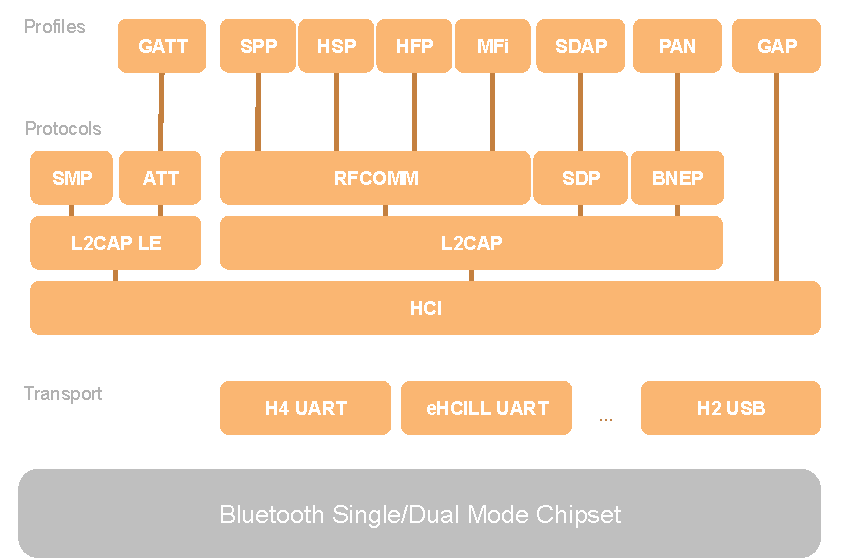
\includegraphics[width=0.9\textwidth]{picts/btstack-protocols.pdf} 
   \caption{BTstack Protocol Architecture}
   \label{fig:BTstackProtocolArchitecture}
\end{figure}

%  As depicted in Figure \ref{fig:BTstackProtocolArchitecture}, BTstack implements following Bluetooth technologies:
% \begin{itemize}
% \item Classic Bluetooth:
% 	\begin{itemize}
% 	\item protocols: HCI, L2CAP, RFCOMM, SDP, BNEP
% 	\item profiles: GAP, SPP, PAN (PAN User (PANU))
% 	\end{itemize}
% \item Bluetooth Low Energy:
% 	\begin{itemize}
% 	\item protocols: HCI, L2CAP-LE, SMP, ATT
% 	\item profiles: GAP-LE, GATT
% 	\end{itemize}
% \end{itemize}

\subsection{HCI - Host Controller Interface}

The HCI protocol provides a command interface to the Bluetooth chipset. In BTstack, the HCI implementation also keeps track of all active connections and also handles the re-assembly of higher layer (L2CAP) packets. Many features of the Generic Access Profile (GAP Classic) can be achieved by sending a single HCI command. Because of this, if there's no special GAP function, please consider sending the HCI command directly, as explained in the following. 

\subsubsection{Defining custom HCI command templates}

Each HCI command is assigned a 2-byte OpCode used to uniquely identify different types of commands. The OpCode parameter is divided into two fields, called the OpCode Group Field (OGF) and OpCode Command Field (OCF), see \BluetoothSpecification{} - Core Version 4.0, Volume 2, Part E, Chapter 5.4. In a HCI command packet, the OpCode is followed by parameter total length, and the actual parameters.

BTstack provides the \emph{hci\_cmd\_t} struct as a compact format to define HCI command packets, see Listing \ref{HCIcmdTemplate},  and \path{include/btstack/hci_cmds.h} file in the source code. The OpCode of a command can be calculated using the OPCODE macro. 


\noindent\begin{minipage}{\textwidth}
\begin{lstlisting}[caption = hci\_cmds.h defines HCI command template., label=HCIcmdTemplate]
// Calculate combined ogf/ocf value.
#define OPCODE(ogf, ocf) (ocf | ogf << 10)

// Compact HCI Command packet description.
typedef struct {
    uint16_t    opcode;
    const char *format;
} hci_cmd_t;

extern const hci_cmd_t hci_write_local_name;
...
\end{lstlisting}
\end{minipage}

\begin{lstlisting}[caption=hci.h defines possible OGFs used for creation of a HCI command., label=hciCmdOGF]
#define OGF_LINK_CONTROL  0x01
#define OGF_LINK_POLICY  0x02
#define OGF_CONTROLLER_BASEBAND  0x03
#define OGF_INFORMATIONAL_PARAMETERS 0x04
#define OGF_LE_CONTROLLER   0x08
#define OGF_BTSTACK  0x3d
#define OGF_VENDOR  0x3f
\end{lstlisting}

Listing \ref{hciCmdOGF} shows the OGFs provided by BTstack in \path{src/hci.h} file.  For all existing Bluetooth commands and their OCFs see \BluetoothSpecificationURL{} - Core Version 4.0, Volume 2, Part E, Chapter 7.

Listing \ref{HCIcmdExample} illustrates the \emph{hci\_write\_local\_name} HCI command template from \mbox{BTstack} library. It uses  OGF\_CONTROLLER\_BASEBAND as OGF, 0x13 as OCF, and has one parameter with format "N" indicating a null terminated UTF-8 string. Table \ref{table:hciformat} lists the format specifiers supported by BTstack. Check \path{src/hci_cmds.c} for other predefined HCI commands and info on their parameters.

\begin{lstlisting}[caption= Example of HCI command template., label=HCIcmdExample]
// Sets local Bluetooth name
const hci_cmd_t hci_write_local_name = {
    OPCODE(OGF_CONTROLLER_BASEBAND, 0x13), "N"
    // Local name (UTF-8, Null Terminated, max 248 octets)
};
\end{lstlisting}

\begin{table*}\centering
\caption{Supported Format Specifiers of HCI Command Parameter}
\begin{tabular}{cl}\toprule
Format Specifier & Description\\ 
\midrule
"1" & 8 bit value \\
"2" & 16 bit value \\
"H" & HCI handle \\
"3" & 24 bit value \\
"4" & 32 bit value \\
"B" & Bluetooth address \\
"D" & 8 byte data block \\
"E" & Extended Inquiry Information 240 octets \\
"N" & UTF8 string, null terminated \\
"P" & 16 byte PIN code or link key \\
"A" & 31 bytes advertising data \\
"S" & Service Record (Data Element Sequence)\\
\bottomrule
\label{table:hciformat}
\end{tabular}
\end{table*}

\subsubsection{Sending  HCI command based on a template}

\begin{lstlisting}[caption= Send hci\_write\_local\_name command that takes a string as a parameter., label=HCIcmdExampleLocalName]
if (hci_can_send_packet_now(HCI_COMMAND_DATA_PACKET)){
    hci_send_cmd(&hci_write_local_name, "BTstack Demo");
}  
\end{lstlisting}

You can use the \emph{hci\_send\_cmd} function to send HCI command based on a template and a list of parameters. However, it is necessary to check that the outgoing packet buffer is empty and that the Bluetooth module is ready to receive the next command - most modern Bluetooth modules only allow  to send a single HCI command. 
This can be done by calling \emph{hci\_can\_send\_command\_packet\_now()} function, which returns true, if it is ok to send.

Listing \ref{HCIcmdExampleLocalName} illustrates how to manually set the device name with the HCI Write Local Name command. 

Please note, that an application rarely has to send HCI commands on its own. Instead, BTstack provides convenience functions in HCI/GAP and higher level protocols use HCI automatically. E.g. to set the name, you can call \emph{gap\_set\_local\_name()} before powering up. The main use of HCI commands in application is during the startup phase to configure special features not available via the GAP API yet.



\subsection{L2CAP -  Logical Link Control and Adaptation Protocol}
The L2CAP protocol supports higher level protocol multiplexing and packet fragmentation. It provides the base for the RFCOMM and BNEP protocols. For all profiles that are officially supported by BTstack, L2CAP does not need to be used directly. For testing or the development of custom protocols, it's helpful to be able to access and provide L2CAP services however.

\subsubsection{Access an L2CAP service on a remote device}
L2CAP is based around the concept of channels. A channel is a logical connection on top of a baseband connection. Each channel is bound to a single protocol in a many-to-one fashion. Multiple channels can be bound to the same protocol, but a channel cannot be bound to multiple protocols. Multiple channels can share the same baseband connection.

\begin{lstlisting}[caption=L2CAP handler for outgoing L2CAP channel.,label=L2CAPremoteService]
btstack_packet_handler_t l2cap_packet_handler;

void btstack_setup(){
    ...
    l2cap_init();
}

void create_outgoing_l2cap_channel(bd_addr_t address, uint16_t psm, uint16_t mtu){
     l2cap_create_channel_internal(NULL, l2cap_packet_handler, remote_bd_addr, psm, mtu);
}

void l2cap_packet_handler(uint8_t packet_type, uint16_t channel, uint8_t *packet, uint16_t size){
    if (packet_type == HCI_EVENT_PACKET &&
          packet[0] == L2CAP_EVENT_CHANNEL_OPENED){
        if (packet[2]) {
            printf("Connection failed\n\r");
            return;
        }
        printf("Connected\n\r");
    }
    if (packet_type == L2CAP_DATA_PACKET){
        // handle L2CAP data packet
        return;
    }
}
\end{lstlisting}

To communicate with an L2CAP service on a remote device, the application on a local Bluetooth device initiates the L2CAP layer using the \emph{l2cap\_init} function, and then creates an outgoing L2CAP channel to the PSM of a remote device using the \emph{l2cap\_create\_channel\_internal} function. The  \emph{l2cap\_-create\_channel\_internal} function will initiate a new baseband connection if it does not already exist. The packet handler that is given as an input parameter of the L2CAP create channel function will be assigned to the new outgoing L2CAP channel. This handler receives the L2CAP\_EVENT\_CHANNEL\_OPENED and L2CAP\_EVENT\_CHAN-NEL\_CLOSED events and L2CAP data packets, as shown in Listing \ref{L2CAPremoteService}.


\subsubsection{Provide an L2CAP service}

To provide an L2CAP service, the application on a local Bluetooth device must init the L2CAP layer and register the service with \emph{l2cap\_register\_service\_internal}. From there on, it can wait for incoming L2CAP connections. The application can accept or deny an incoming connection by calling the \emph{l2cap\_accept\_connection\_internal} and \emph{l2cap\_deny\_connection\_internal} functions respectively. If a connection is accepted and the incoming L2CAP channel gets successfully opened, the L2CAP service can send L2CAP data packets to the connected device with \emph{l2cap\_send\_internal}. 

\begin{lstlisting}[caption=Providing an L2CAP service., label=L2CAPService]
void btstack_setup(){
    ...
    l2cap_init();
    l2cap_register_service_internal(NULL, packet_handler, 0x11,100);
}

void packet_handler (uint8_t packet_type, uint16_t channel, uint8_t *packet, uint16_t size){
      ...
      if (packet_type == L2CAP_DATA_PACKET){
        // handle L2CAP data packet
        return;
    }
    switch(event){
        ...
        case L2CAP_EVENT_INCOMING_CONNECTION:
            bt_flip_addr(event_addr, &packet[2]);
            handle     = READ_BT_16(packet, 8); 
            psm        = READ_BT_16(packet, 10); 
            local_cid  = READ_BT_16(packet, 12); 
            printf("L2CAP incoming connection requested.");
            l2cap_accept_connection_internal(local_cid);
            break;
        case L2CAP_EVENT_CHANNEL_OPENED:
            bt_flip_addr(event_addr, &packet[3]);
            psm = READ_BT_16(packet, 11); 
            local_cid = READ_BT_16(packet, 13); 
            handle = READ_BT_16(packet, 9);
            if (packet[2] == 0) {
                printf("Channel successfully opened.");
            } else {
                printf("L2CAP connection failed. status code.");
            }
            break;        
        case L2CAP_EVENT_CREDITS:
        case DAEMON_EVENT_HCI_PACKET_SENT:
            tryToSend();
            break;
        case L2CAP_EVENT_CHANNEL_CLOSED:
            break;
    }
}
\end{lstlisting}

Sending of L2CAP data packets may fail due to a full internal BTstack outgoing packet buffer, or if the ACL buffers in the Bluetooth module become full, i.e., if the application is sending faster than the packets can be transferred over the air. In such case, the application can try sending again upon reception of DAEMON\_EVENT\_HCI\_PACKET\_SENT or L2CAP\_EVENT\_CREDITS event. The first event signals that the internal BTstack outgoing buffer became free again, the second one signals the same for ACL buffers in the Bluetooth chipset. Listing \ref{L2CAPService} provides L2CAP service example code.

\todo{\textbf{L2CAP and Security Levels}} \\

\subsubsection{L2CAP LE - L2CAP Low Energy Protocol}
In addition to the full L2CAP implementation in the \emph{src} folder, BTstack provides an optimized v\emph{l2cap\_le} implementation in the \emph{ble} folder. This L2CAP LE variant can be used for single-mode devices and provides the base for the ATT and SMP protocols.



\subsection{RFCOMM - Radio Frequency Communication Protocol}
%\label{section:flowcontrol}
The Radio frequency communication (RFCOMM) protocol provides emulation of serial ports over the L2CAP protocol.
and reassembly. It is the base for the Serial Port Profile and other profiles used for telecommunication like Head-Set Profile, Hands-Free Profile, Object Exchange (OBEX) etc.

\subsubsection{RFCOMM flow control.}
RFCOMM has a mandatory credit-based flow-control. This means that two devices that established RFCOMM connection, use credits to keep track of how many more RFCOMM data packets can be sent to each. If a device has no (outgoing) credits left, it cannot send another RFCOMM packet, the transmission must be paused. During the connection establishment, initial credits are provided. BTstack tracks the number of credits in both directions. If no outgoing credits are available, the RFCOMM send function will return an error, and you can try later. For incoming data, BTstack provides channels and services with and without automatic credit management via different functions to create/register them respectively. If the management of credits is automatic, the new credits are provided when needed relying on ACL flow control - this is only useful if there is not much data transmitted and/or only one physical connection is used. If the management of credits is manual, credits are provided by the application such that it can manage its receive buffers explicitly. 

\todo{\textbf{RFCOMM port configuration for both local and remote}}\\
\todo{\textbf{RFCOMM  modem and line status control/information}}\\
\todo{\textbf{RFCOMM\_AGGREGATE\_FLOW\_OFF example}}\\
\todo{\textbf{RFCOMM and Security Levels}}\\

\subsubsection{Access an RFCOMM service on a remote device}

To communicate with an RFCOMM service on a remote device, the application on a local Bluetooth device initiates the RFCOMM layer using the \emph{rfcomm\_init} function, and then creates an outgoing RFCOMM channel to a given server channel on a remote device using the \emph{rfcomm\_create\_channel\_internal} function. The  \emph{rfcomm\_create\_channel\_intern-al} function will initiate a new L2CAP connection for the RFCOMM multiplexer, if it does not already exist. The channel will automatically provide enough credits to the remote side. To provide credits manually, you have to create the RFCOMM connection by calling \emph{rfcomm\_create\_channel\_with\_initial\_credits\_internal} - see Section \ref{sec:manualCredits}.


The packet handler that is given as an input parameter of the RFCOMM create channel function will be assigned to the new outgoing \mbox{RFCOMM} channel. This handler receives the RFCOMM\_EVENT\_OPEN\_CHAN-NEL\_COMPLETE and RFCOMM\_EVENT\_CHANNEL\_CLOSED events, and RFCOMM data packets, as shown in Listing \ref{RFCOMMremoteService}.

\subsubsection{Provide an RFCOMM service}
\label{section:rfcomm_service}

To provide an RFCOMM service, the application on a local Bluetooth device must first init the L2CAP and RFCOMM layers and then register the service with \emph{rfcomm\_register\_service\_internal}. From there on, it can wait for incoming RFCOMM connections. The application can accept or deny an incoming connection by calling the \emph{rfcomm\_accept\_connection-\_internal} and \emph{rfcomm\_deny\_connection\_internal} functions respectively. If a connection is accepted and the incoming RFCOMM channel gets successfully opened, the RFCOMM service can send RFCOMM data packets to the connected device with \emph{rfcomm\_send\_internal} and receive data packets by the packet handler provided by the \emph{rfcomm\_register\_service\_internal} call.

Sending of RFCOMM data packets may fail due to a full internal BTstack outgoing packet buffer, or if the ACL buffers in the Bluetooth module become full, i.e., if the application is sending faster than the packets can be transferred over the air. In such case, the application can try sending again upon reception of DAEMON\_EVENT\_HCI\_PACKET\_SENT or RFCOMM\_EVENT\_CREDITS event. The first event signals that the internal BTstack outgoing buffer became free again, the second one signals that the remote side allowed to send another  packet. Listing \ref{RFCOMMService} provides the RFCOMM service example code.

\begin{lstlisting}[caption= RFCOMM service with automatic credit management. , label=automaticFlowControl]
void btstack_setup(void){
    ...
    // init RFCOMM
    rfcomm_init();
    rfcomm_register_packet_handler(packet_handler);
    rfcomm_register_service_internal(NULL, rfcomm_channel_nr, 100); 
}
\end{lstlisting}


\subsubsection{Living with a single output buffer}
\label{section:single_buffer}
% l2cap checks hci_can_send_packet now
Outgoing packets, both commands and data, are not queued in BTstack. This section explains the consequences of this design decision for sending data and why it is not as bad as it sounds.

\noindent\begin{minipage}{\textwidth}
\begin{lstlisting}[caption=Preparing and sending data., label=SingleOutputBufferTryToSend]
void prepareData(void){
    ...
}

void tryToSend(void){
    if (!dataLen) return;
    if (!rfcomm_channel_id) return;
    
    int err = rfcomm_send_internal(rfcomm_channel_id,  dataBuffer, dataLen);
    switch (err){
        case 0:
            // packet is sent prepare next one
            prepareData();
            break;
        case RFCOMM_NO_OUTGOING_CREDITS:
        case BTSTACK_ACL_BUFFERS_FULL:
            break;
        default:
           printf("rfcomm_send_internal() -> err %d\n\r", err);
        break;
    }
}
\end{lstlisting}
\begin{lstlisting}[ caption= Managing the speed of RFCOMM packet generation., label=SingleOutputBufferTryPH]
void packet_handler (uint8_t packet_type, uint16_t channel, uint8_t *packet, uint16_t size){
    ...
    switch(event){
        case RFCOMM_EVENT_OPEN_CHANNEL_COMPLETE:
            if (status) {
                printf("RFCOMM channel open failed.");
            } else {
                rfcomm_channel_id = READ_BT_16(packet, 12);
                rfcomm_mtu = READ_BT_16(packet, 14);
                printf("RFCOMM channel opened, mtu = %u.", rfcomm_mtu);
            }
            break;
        case RFCOMM_EVENT_CREDITS:
        case DAEMON_EVENT_HCI_PACKET_SENT:
            tryToSend();
            break;
        case RFCOMM_EVENT_CHANNEL_CLOSED:
            rfcomm_channel_id = 0;
            break;
       ...
       }
}
\end{lstlisting}
\end{minipage}

Independent from the number of output buffers, packet generation has to be adapted to the remote receiver and/or maximal link speed. Therefore, a packet can only be generated when it can get sent. With this assumption, the single output buffer design does not impose additional restrictions. In the following, we show how this is used for adapting the RFCOMM send rate. 

BTstack returns BTSTACK\_ACL\_BUFFERS\_FULL, if the outgoing buffer is full and RFCOMM\_NO\_OUTGOING\_CREDITS, if no outgoing credits are available. In Listing \ref{SingleOutputBufferTryToSend}, we show how to resend data packets when credits or outgoing buffers become available.


RFCOMM's mandatory credit-based flow-control imposes an additional constraint on sending a data packet - at least one new RFCOMM credit must be available. BTstack signals the availability of a credit by sending an RFCOMM credit (RFCOMM\_EVENT\_CREDITS) event. 

These two events represent two orthogonal mechanisms that deal with flow control. Taking these mechanisms in account, the application should try to send data packets when one of these two events is received, see Listing \ref{SingleOutputBufferTryPH} for a RFCOMM example.


If the management of credits is manual, credits are provided by the application such that it can manage its receive buffers explicitly, see Listing \ref{explicitFlowControl}.

Manual credit management is recommended when received RFCOMM data cannot be processed immediately. In the SPP flow control example in Section \ref{example:spp_flow_control}, delayed processing of received data is simulated with the help of a periodic timer. To provide new credits, you call the \emph{rfcomm\_grant\_credits} function with the RFCOMM channel ID and the number of credits as shown in Listing \ref{NewCredits}.
Please note that providing single credits effectively reduces the credit-based (sliding window) flow control to a stop-and-wait flow-control that limits the data throughput substantially. On the plus side, it allows for a minimal memory footprint. If possible, multiple RFCOMM buffers should be used to avoid pauses while the sender has to wait for a new credit.


\subsubsection{Slowing down RFCOMM data reception}
\label{sec:manualCredits}
RFCOMM's credit-based flow-control can be used to adapt, i.e., slow down the RFCOMM data to your processing speed. 
For incoming data, BTstack provides channels and services with and without automatic credit management. 
If the management of credits is automatic, see Listing \ref{automaticFlowControl},  new credits are provided when needed relying on ACL flow control. This is only useful if there is not much data transmitted and/or only one physical connection is used


\begin{lstlisting}[float, caption=RFCOMM handler for outgoing RFCOMM channel., label=RFCOMMremoteService] 
void init_rfcomm(){
    ...
    rfcomm_init();
    rfcomm_register_packet_handler(packet_handler);
}

void create_rfcomm_channel(uint8_t packet_type, uint8_t *packet, uint16_t size){
    rfcomm_create_channel_internal(connection, addr, rfcomm_channel);
}

void rfcomm_packet_handler(uint8_t packet_type, uint16_t channel, uint8_t *packet, uint16_t size){
    if (packet_type == HCI_EVENT_PACKET && packet[0] == RFCOMM_EVENT_OPEN_CHANNEL_COMPLETE){
        if (packet[2]) {
            printf("Connection failed\n\r");
            return;
        }
        printf("Connected\n\r");
    }
    
    if (packet_type == RFCOMM_DATA_PACKET){
        // handle RFCOMM data packets
        return;
    }
}
\end{lstlisting}

\begin{lstlisting}[float, caption=Providing RFCOMM service., label=RFCOMMService]
void btstack_setup(){
    ...
    rfcomm_init();
    rfcomm_register_service_internal(NULL, rfcomm_channel_nr, mtu); 
}

void packet_handler(uint8_t packet_type, uint8_t *packet, uint16_t size){
    if (packet_type == RFCOMM_DATA_PACKET){
        // handle RFCOMM data packets
        return;
    }
    ...
    switch (event) {
        ...
        case RFCOMM_EVENT_INCOMING_CONNECTION:
            //data: event(8), len(8), address(48), channel(8), rfcomm_cid(16)
            bt_flip_addr(event_addr, &packet[2]); 
            rfcomm_channel_nr = packet[8];
            rfcomm_channel_id = READ_BT_16(packet, 9);
            rfcomm_accept_connection_internal(rfcomm_channel_id);
            break;
        case RFCOMM_EVENT_OPEN_CHANNEL_COMPLETE:
           // data: event(8), len(8), status (8), address (48), handle(16), server channel(8), rfcomm_cid(16), max frame size(16)
            if (packet[2]) {
                printf("RFCOMM channel open failed.");
                break;
            } 
           // data: event(8), len(8), status (8), address (48), handle (16), server channel(8), rfcomm_cid(16), max frame size(16)
           rfcomm_channel_id = READ_BT_16(packet, 12);
           mtu = READ_BT_16(packet, 14);
           printf("RFCOMM channel open succeeded.");
           break;
        case RFCOMM_EVENT_CREDITS:
        case DAEMON_EVENT_HCI_PACKET_SENT:
            tryToSend();
            break;

        case RFCOMM_EVENT_CHANNEL_CLOSED:
            printf("Channel closed.");
            rfcomm_channel_id = 0;
        break;
    }
}
\end{lstlisting}


% \noindent\begin{minipage}\textwidth
\begin{lstlisting}[ caption= RFCOMM service with manual credit management. , label=explicitFlowControl]
void btstack_setup(void){
    ...
    // init RFCOMM
    rfcomm_init();
    rfcomm_register_packet_handler(packet_handler);
    // reserved channel, mtu=100, 1 credit
    rfcomm_register_service_with_initial_credits_internal(NULL, rfcomm_channel_nr, 100, 1);  
}
\end{lstlisting}

\begin{lstlisting}[caption= Providing new credits , label=NewCredits]
void processing(){
    // process incoming data packet
    ... 
    // provide new credit
    rfcomm_grant_credits(rfcomm_channel_id, 1);
}
\end{lstlisting}

\subsection{SDP - Service Discovery Protocol}
The SDP protocol allows to announce services and discover services provided by a remote Bluetooth device. 

\subsubsection{Create and announce SDP records}
BTstack contains a complete SDP server and allows to register SDP records. An SDP record is a list of SDP Attribute \emph{\{ID, Value\}} pairs that are stored in a Data Element Sequence (DES). The Attribute ID is a 16-bit number, the value can be of other simple types like integers or strings or can itselff contain other DES. 


To create an SDP record for an SPP service, you can call \emph{sdp\_create\_spp\_service} from \path{src/sdp_util.c} with a pointer to a buffer to store the record, the \mbox{RFCOMM} server channel number, and a record name. 

For other types of records, you can use the other functions in \path{src/sdp_util.c}, using the data element \emph{de\_*} functions.  Listing \ref{sdpCreate} shows how an SDP record containing two SDP attributes can be created. First, a DES is created and then the Service Record Handle and Service Class ID List attributes are added to it. The Service Record Handle attribute is added by calling the \emph{de\_add\_number} function twice: the first time to add 0x0000 as attribute ID, and the second time to add the actual record handle (here 0x1000) as attribute value. The Service Class ID List attribute has ID 0x0001, and it requires a list of UUIDs as attribute value. To create the list, \emph{de\_push\_sequence} is called, which "opens" a sub-DES. The returned pointer is used to add elements to this sub-DES. After adding all UUIDs, the sub-DES is "closed" with \emph{de\_pop\_sequence}.

\subsubsection{Query remote SDP service}

BTstack provides an SDP client to query SDP services of a remote device. The SDP Client API  is shown in Appendix \ref{appendix:api_sdp_client}. The \emph{sdp\_client\_query} function initiates an L2CAP connection to the remote SDP server. Upon connect, a \emph{Service Search Attribute} request with a \emph{Service Search Pattern} and a \emph{Attribute ID List} is sent. The result of the \emph{Service Search Attribute} query contains a list of \emph{Service Records}, and each of them contains the requested attributes. These records are handled by the SDP parser. The parser delivers SDP\_PARSER\_ATTRIBUTE\_VALUE and SDP\_PARSER\_COMPLETE events via a registered callback. The SDP\_PARSER\_ATTRIBUTE\_VALUE event delivers the attribute value byte by byte.

On top of this, you can implement specific SDP queries. For example, BTstack provides a query for RFCOMM service name and channel number. This information is needed, e.g., if you want to connect to a remote SPP service. The query delivers all matching RFCOMM services, including its name and the channel number, as well as a query complete  event via a registered callback, as shown in Listing \ref{SDPClientRFCOMM}.

\begin{lstlisting}[caption=Searching RFCOMM services on a remote device., label=SDPClientRFCOMM ]
bd_addr_t remote = {0x04,0x0C,0xCE,0xE4,0x85,0xD3};

void packet_handler (void * connection, uint8_t packet_type, uint16_t channel, uint8_t *packet, uint16_t size){
    if (packet_type != HCI_EVENT_PACKET) return;

    uint8_t event = packet[0];
    switch (event) {
        case BTSTACK_EVENT_STATE:
            // bt stack activated, get started 
            if (packet[2] == HCI_STATE_WORKING){
            	  sdp_query_rfcomm_channel_and_name_for_uuid(remote, 0x0003);
            }
            break;
        default:
            break;
    }
}

static void btstack_setup(){
   ...
    // init L2CAP
    l2cap_init();
    l2cap_register_packet_handler(packet_handler);
}

void handle_query_rfcomm_event(sdp_query_event_t * event, void * context){
    sdp_query_rfcomm_service_event_t * ve;
            
    switch (event->type){
        case SDP_QUERY_RFCOMM_SERVICE:
            ve = (sdp_query_rfcomm_service_event_t*) event;
            printf("Service name: '%s', RFCOMM port %u\n", ve->service_name, ve->channel_nr);
            break;
        case SDP_QUERY_COMPLETE:
            report_found_services();
            printf("Client query response done with status %d. \n", ce->status);
            break;
    }
}

int main(void){
    hw_setup();
    btstack_setup();
    
    // register callback to receive matching RFCOMM Services and 
    // query complete event 
    sdp_query_rfcomm_register_callback(handle_query_rfcomm_event, NULL);

    // turn on!
    hci_power_control(HCI_POWER_ON);
    // go!
    run_loop_execute(); 
    return 0;
}

\end{lstlisting}

\begin{lstlisting}[caption=Creating record with the data element (\emph{de\_*}) functions., label=sdpCreate]
uint8_t des_buffer[200];
uint8_t* attribute;
de_create_sequence(service);
    
// 0x0000 "Service Record Handle"
de_add_number(des_buffer, DE_UINT, DE_SIZE_16, SDP_ServiceRecordHandle);
de_add_number(des_buffer, DE_UINT, DE_SIZE_32, 0x10001);
    
// 0x0001 "Service Class ID List"
de_add_number(des_buffer,  DE_UINT, DE_SIZE_16, SDP_ServiceClassIDList);
attribute = de_push_sequence(des_buffer);
{
    de_add_number(attribute,  DE_UUID, DE_SIZE_16, 0x1101 );
}
de_pop_sequence(des_buffer, attribute);
\end{lstlisting}
% \end{minipage}

\subsection{BNEP -  Bluetooth Network Encapsulation Protocol}
The BNEP protocol is built on top of L2CAP and it is used to transport control and data packets over standard network protocols such as TCP, IPv4 or IPv6.  BNEP specifies a minimum L2CAP MTU of 1691. 

To receive BNEP events, please register a packet handler with \emph{bnep\_register\_packet\_handler}.

\subsubsection{Access a BNEP service on a remote device}
To connect to a remote BNEP service, you need to know its UUID. The set of available UUIDs can be queried by a SDP query for the PAN profile. Please see section \ref{section:pan_profile} for details. With the remote UUID, you can create a connection using the \emph{bnep\_connect} function. You'll receive a \emph{BNEP\_EVENT\_OPEN\_CHANNEL\_COMPLETE} on success or failure. 

If the connection was opened successfully, you can send ethernet packets  if you can send a Ethernet frames by first checking \emph{bnep\_can\_send\_packet\_now} and then calling \emph{bnep\_send}. You'll receive Ethernet frames via the registered packet handler and a packet type of \emph{BNEP\_DATA\_PACKET}.

BTstack BNEP implementation supports both network protocol filter and multicast filters with \emph{bnep\_set\_net\_type\_filter} and \emph{bnep\_set\_multicast\_filter} respectively.

Finally, to close a BNEP connection, you can call \emph{bnep\_disconnect}

\subsubsection{Provide BNEP service}
You can also provide a BNEP service by calling \emph{bnep\_register\_service} with the provided service UUID and a max frame size.

After an incoming connection was established, a \emph{BNEP\_EVENT\_INCOMING\_CONNECTION} event is received. Ethernet packets can now be sent and received as in the previous section.

\subsection{ATT - Attribute Protocol}
ATT is a wire application protocol, while GATT dictates how ATT is employed in service composition. Every Low Energy profile must be based on GATT. So, ultimately, every LE service uses ATT as the application protocol. An ATT server stores attributes. An ATT client stores nothing; it uses the ATT wire protocol to read and write values on server attributes. Most of the ATT protocol is pure client-server: client takes the initiative, server answers. But ATT has notification and indication capabilities, in which the server takes the initiative of notifying a client that an attribute value has changed, saving the client from having to poll the attribute.

\todo{\textbf{Explain ATT Client and Server.}} \\
\todo{\textbf{Explain how to setup ATT Database}} \\

\subsection{SMP - Security Manager Protocol }
The SMP protocol allows to setup authenticated and encrypted connection.

\todo{\textbf{Explain SMP and what you can do with it, what it does for you}} \\


% \newcommand{\FreeBSDHandbook}{\urlfoot{http://www.freebsd.org/doc/en\_US.ISO8859-1/books/handbook/network-bluetooth.html}{FreeBSD Handbook}}

\section{Profiles}
As promised in the previous chapter, we explain how to implement various Bluetooth profiles in this one.


\subsection{GAP - Generic Access Profile: Classic}

\subsubsection{Become discoverable}
A remote unconnected Bluetooth device must be set as "discoverable" in order to be seen by a device performing the inquiry scan. To become discoverable, an application can call \emph{hci\_discoverable\_control}  with input parameter 1. If you want to provide a helpful name for your device, the application can set its local name by sending the $hci\_write\_local\_name$ command. To save energy, you may set the device as undiscoverable again, once a connection is established. See Listing \ref{Discoverable} for an example.

\begin{lstlisting}[caption=Setting device as discoverable. OFF by default., label=Discoverable]
int main(void){
    ... 
    // make discoverable
    hci_discoverable_control(1);
    run_loop_execute(); 
    return 0;
}
void packet_handler (uint8_t packet_type, uint8_t *packet, uint16_t size){
     ...
     switch(state){
          case INIT:
              if (packet[2] == HCI_STATE_WORKING) {
                  hci_send_cmd(&hci_write_local_name, "BTstack SPP Counter");
                  state = W4_CONNECTION;
               }
              break;
          case W4_CHANNEL_COMPLETE:
              // if connection is successful, make device undiscoverable
              hci_discoverable_control(0);
          ...
     }
 }
\end{lstlisting}


\subsubsection{Discover remote devices}
\label{section:DiscoverDevices}
To scan for remote devices, the \emph{hci\_inquiry} command is used. After that, the Bluetooth devices actively scans for other devices and reports these as part of HCI\_EVENT\_INQUIRY\_RESULT, HCI\_EVENT-\_INQUIRY\_RESULT\_WITH\_RSSI, or HCI\_EVENT\_EXTENDED\_INQUIRY\_RE-SPONSE events. Each response contains at least the Bluetooth address, the class of device, the page scan repetition mode, and the clock offset of found device. The latter events add information about the received signal strength or provide the Extended Inquiry Result (EIR). A code snippet is shown in Listing \ref{DiscoverDevices}.

By default, neither RSSI values nor EIR are reported. If the Bluetooth device implements Bluetooth Specification 2.1 or higher, the \emph{hci\_write\_inquiry\_mode} command enables reporting of this advanced features (0 for standard results, 1 for RSSI, 2 for RSSI and EIR). 

A complete GAP inquiry example is provided in Section \ref{example:GapInquiry}.

\begin{lstlisting}[float, caption=Discovering remote Bluetooth devices., label=DiscoverDevices]
void print_inquiry_results(uint8_t *packet){
    int event = packet[0];
    int numResponses = packet[2];
    uint16_t classOfDevice, clockOffset;
    uint8_t  rssi, pageScanRepetitionMode;
    for (i=0; i<numResponses; i++){
        bt_flip_addr(addr, &packet[3+i*6]);
        pageScanRepetitionMode = packet [3 + numResponses*6 + i];
        if (event == HCI_EVENT_INQUIRY_RESULT){
            classOfDevice = READ_BT_24(packet, 3 + numResponses*(6+1+1+1) + i*3);
            clockOffset =   READ_BT_16(packet, 3 + numResponses*(6+1+1+1+3) + i*2) & 0x7fff;
            rssi  = 0;
        } else {
            classOfDevice = READ_BT_24(packet, 3 + numResponses*(6+1+1)     + i*3);
            clockOffset =   READ_BT_16(packet, 3 + numResponses*(6+1+1+3)   + i*2) & 0x7fff;
            rssi  = packet [3 + numResponses*(6+1+1+3+2) + i*1];
        }
        printf("Device found: %s with COD: 0x%06x, pageScan %u, clock offset 0x%04x, rssi 0x%02x\n", bd_addr_to_str(addr), classOfDevice, pageScanRepetitionMode, clockOffset, rssi);
    }
}

void packet_handler (uint8_t packet_type, uint8_t *packet, uint16_t size){
    ...
    switch (event) {
         case HCI_STATE_WORKING:
            hci_send_cmd(&hci_write_inquiry_mode, 0x01); // with RSSI
            break;
        case HCI_EVENT_COMMAND_COMPLETE:
            if (COMMAND_COMPLETE_EVENT(packet, hci_write_inquiry_mode) ) {
                start_scan();
            }
        case HCI_EVENT_COMMAND_STATUS:
            if (COMMAND_STATUS_EVENT(packet, hci_write_inquiry_mode) ) {
                printf("Ignoring error (0x%x) from hci_write_inquiry_mode.\n", packet[2]);
                hci_send_cmd(&hci_inquiry, HCI_INQUIRY_LAP, INQUIRY_INTERVAL, 0);
            }
            break;
        case HCI_EVENT_INQUIRY_RESULT:
        case HCI_EVENT_INQUIRY_RESULT_WITH_RSSI:
            print_inquiry_results(packet);
            break;
       ...
    }
}
\end{lstlisting}

\begin{lstlisting}[caption=Answering authentication request with PIN 0000., label=PinCodeRequest]
void packet_handler (uint8_t packet_type, uint8_t *packet, uint16_t size){
    ...
    switch (event) {
        case HCI_EVENT_PIN_CODE_REQUEST:
            // inform about pin code request
            printf("Pin code request - using '0000'\n\r");
            bt_flip_addr(bd_addr, &packet[2]);
            
            // baseband address, pin length, PIN: c-string
            hci_send_cmd(&hci_pin_code_request_reply, &bd_addr, 4, "0000");
            break;
       ...
    }
}
\end{lstlisting}
\subsubsection{Pairing of devices}
By default, Bluetooth communication is not authenticated, and any device can talk to any other device. A Bluetooth device (for example, cellular phone) may choose to require authentication to provide a particular service (for example, a Dial-Up service). The process of establishing authentication is called pairing. Bluetooth provides two mechanism for this.

On Bluetooth devices that conform to the Bluetooth v2.0 or older specification, a PIN code (up to 16 bytes ASCII) has to be entered on both sides. This isn't optimal for embedded systems that do not have full I/O capabilities. To support pairing with older devices using a PIN, see Listing \ref{PinCodeRequest}.

The Bluetooth v2.1 specification introduces Secure Simple Pairing (SSP), which is a better approach as it both improves security and is better adapted to embedded system. With SSP, the devices first exchange their IO Capabilities and then settle on one of several ways to verify that the pairing is legitimate. If the Bluetooth device supports SSP, BTstack enables it by default and even automatically accepts SSP pairing requests. Depending on the product in which BTstack is used, this may not be desired and should be replaced with code to interact with the user.

Regardless of the authentication mechanism (PIN/SSP), on success, both devices will generate a link key. The link key can be stored either in the Bluetooth module itself or in a persistent storage, see Section \ref{section:persistent_storage}. The next time the device connect and request an authenticated connection, both devices can use the previously generated link key. Please note that the pairing must be repeated if the link key is lost by one device.

\todo{\textbf{Dedicated bonding.}} \\



\subsection{SPP - Serial Port Profile}
The SPP profile defines how to set up virtual serial ports and connect two Bluetooth enabled devices. See Appendix \ref{appendix:api_} for the SPP API.

\todo{\textbf{Explain SPP use.}} \\


\subsection{PAN -  Personal Area Networking Profile}
The PAN profile uses BNEP to provide on-demand networking capabilities between Bluetooth devices. The PAN profile defines the following roles:
\begin{itemize}
\item PAN User (PANU)
\item Network Access Point (NAP)
\item Group Ad-hoc Network (GN)
\end{itemize}

PANU is a Bluetooth device that communicates as a client with GN, or NAP, or with another PANU Bluetooth device, through a point-to-point connection. Either the PANU or the other Bluetooth device may terminate the connection at anytime.

NAP is a Bluetooth device that provides the service of routing network packets between PANU by using BNEP and the IP routing mechanism. A NAP can also act as a bridge between Bluetooth networks and other network technologies by using the Ethernet packets.

The GN role enables two or more PANUs to interact with each other through a wireless network without using additional networking hardware. The devices are connected in a piconet where the GN acts as a master and communicates either point-to-point or a point-to-multipoint with a maximum of seven PANU slaves by using BNEP.

Currently, BTstack supports only PANU.

\subsection{GAP - Generic Access Profile: Low Energy}
The GAP profile defines how to discover and how to connect to a Bluetooth device. There are several GAP roles that a Bluetooth device can take, but the most important ones are the Central and the Peripheral role. Peripheral devices are those that provide information or can be controlled and central devices are those that consume information or control the peripherals. Before the connection can be established, devices are first going through the advertising process. What happens with the peripheral device after the central device connect to a it, depends on the peripheral's Bluetooth controller. The peripheral will either stop advertising itself and other devices will no longer be able to see it or connect to it until the existing connection is broken, or it will be able to continue with advertising so that the parallel connections can be established.

% \subsection{Low Energy}
The focus is on two different device roles:  devices that provide services and/or can be controlled and devices that consume services and/or control other devices. Devices are first going through the advertising process that is governed by the Generic Access Profile (GAP). Once the connection is established, the communication will be governed by the Generic Attribute Profile (GATT). Both profiles, GAP and GATT, have concepts that describe these two BLE roles:  GAP defines Peripheral and Central, and GATT defines Server and Client role respectively. The GATT roles are not necessarily tied to specific GAP roles and may be specified by higher layer profiles. GATT is built on top of the Attribute Protocol (ATT), which defines how to discover, read, and write attributes on a peer device. In addition, BLE uses two more BT protocols: SMP for for pairing and transport specific key distribution and L2CAP LE variant optimized for connectionless data used by Bluetooth Low Energy devices. 

\textbf{Private/random addresses.}
To better protect privacy, a LE device can choose use a private i.e. random Bluetooth address. This address changes at a user-specified rate. To allow for later reconnection, the central and peripheral devices exchange their Identity Resolving Keys (IRKs) during bonding. The IRK is used to verify if a new address belongs to a previously bonded device.

\textbf{GAP BLE Roles.}
There are four GAP roles defined for a Bluetooth low energy device: Broadcaster, Observer, Peripheral and Central. A device may operate in multiple GAP roles concurrently.
\begin{itemize}
\item \emph{GAP Broadcaster Role} - A broadcast device only sends advertisements and cannot be connected. It can emit some useful data as part of the advertisement. The most prominent use for this is Apple's iBeacon technology which uses broadcast devices to emit a unique ID. Apple's iOS framework then help to map this ID onto a specific location, e.g., in a museum. Broadcasting is efficient as no connection and no ATT database are needed. To control energy consumption the broadcast interval can be configured. An advertisement can contain up to 31 bytes of information. In addition, another 31 bytes of information can be sent in the scan response.
\item \emph{GAP Observer Role} - An observer device only receives advertising events and cannot be connected. 
\item \emph{GAP Central Role} - The role of the central device is to scan for peripherals, connect to them, and discover and receive data from them or sends data to control them. During scanning the central device can retrieve information on other device such are its name and unique number, as well as some broadcast data from its services. Upon connection, the central explores the device by discovering its primary and included services, characteristics, and characteristic descriptors.
\item \emph{GAP Peripheral Role} - The role of a peripheral device is to deliver information on their inputs, i.e. sensor values, battery level, current time, to the applications running on central devices. It can also receive a write request from a central device and control connected actors, e.g. turn on and set the color of the light. Peripherals can broadcast data, they can be discovered and connected to by a central device, they can stay also disconnected and then establish connection when needed. 
\end{itemize} 

\textbf{Advertising and Scan Response Data.}
There are two ways to send advertising out with GAP: The Advertising Data payload and the Scan Response payload. Both payloads are identical and can contain up to 31 bytes of data, but only the advertising data payload is mandatory. The scan response payload is an optional secondary payload that central devices can request.

\subsection{GATT - Generic Attribute Profile}
The GATT profile uses the ATT for discovering services, and for reading and writing characteristic values on a peer device. GATT also specifies the format of data contained on the GATT server: it groups ATT attributes into Services and Characteristics, and defines set of queries the GATT Client can use to discover services, characteristics.

\textbf{GATT LE Roles.}
There are two GATT roles defined for a Bluetooth low energy device:
\begin{itemize}
\item \emph{GATT Server Role} - The GATT server stores the data and accepts GATT client requests, commands and confirmations. The GATT server sends responses to requests and when configured, sends indication and notifications asynchronously to the GATT client. 
\item \emph{GATT Client Role} - The GATT Client is used to discover services, and their characteristics and descriptors on a peer device. It can also subscribe for notifications or indications that the characteristic on the GATT server has changed its value. 
\end{itemize}

\textbf{Attribute Database - GATT-based Profile Hierarchy.}
Attributes, as transported by the Attribute Protocol, are formatted as services and characteristics. Services may contain a collection of characteristics. Characteristics contain a single value and any number of descriptors describing the characteristic value. The peripheral device server (ATT server) provides a set of attributes that are stored in a simple lookup database. GATT formats these attributes as services and characteristics. Services may contain a collection of characteristics. Characteristics contain a single value and any number of descriptors describing the characteristic value. A service starts with a service declaration attribute defining its type, i.e. primary or secondary. It is followed by the included services and characteristics. By means of including services, the service can incorporate more complex behavior, and still keep the definition small. A characteristic is assigned to a single value that can be accessed. It is composed of three basic elements: declaration, value and descriptors. The characteristic declaration defines how the data can be accessed. A characteristic descriptor is used to capture the additional properties, e.g., to configure if the characteristic value should be reported upon its change. Together, characteristic declaration and the descriptors define types of action that can be performed on characteristic value.

The security that is required to access a service or a characteristic is defined in ATT database along with service/characteristic declaration. The GATT Server usually does not initiate any security request, but it can. 




\pagebreak
\section{Examples}

\label{examples}
The \path{MSP-EXP430F5438-CC256x} folder in BTstack repository currently includes the following examples for the MSP430F5438 Experimenter Board:
\begin{itemize}
\item UART example:
    \begin{itemize}
    \item \emph{led\_counter}: provides UART and timer interrupt without Bluetooth.
    \end{itemize}
\item GAP example:
    \begin{itemize}
    \item \emph{gap\_inquiry}: uses GAP to discover surrounding Bluetooth devices and then requests their remote name.
    \end{itemize}
\item SPP Server examples :
    \begin{itemize}
    \item \emph{spp\_counter}: provides a virtual serial port via SPP and a periodic timer over RFCOMM. 
    \item \emph{spp\_accel}: provides a virtual serial port via SPP. On connect, it sends the current accelerometer values as fast as possible.
    \item \emph{spp\_flowcontrol}: provides a virtual serial port via SPP with manual RFCOMM credit management. Delayed processing of received data is simulated with the help of a periodic timer. 
    \end{itemize}
% \item SPP Client example: requires an SDP client to query SPP RFCOMM channel number. It is not yet provided by BTstack. Outgoing RFCOMM connections are fully supported otherwise.
\item HID Host example:
    \begin{itemize}                                    
    \item \emph{hid\_demo}: on start, the device does a device discovery and connects to the first Bluetooth keyboard it finds, pairs, and allows to type on the little LCD screen. 
%   \item \emph{mouse}: on start, the device does a device discovery and connects to the first Bluetooth keyboard it finds, paris, and allows move cursor on the screen. It is not yet provided by BTstack, but it can be created by combining existing parts.
    \end{itemize}
%\item HID Device examples:
%   \begin{itemize}
%   \item \emph{keyboard}: a keyboard device is simulated. Pressing the two buttons on the EXP430 board are mapped to Space and Enter. It is not yet provided by BTstack. %-- version for different board exists, needs to handle button IRQs
%   \end{itemize}
\item Low Energy example:
    \begin{itemize}
    \item \emph{ble\_server}: provides a ready-to-run example for a test Peripheral device. It assumes that a PAN1323 or 1326 module with a CC2564 chipset is used.
    \item \emph{gatt\_browser}: shows how to use the GATT Client API to discover primary services and their characteristics.
    \end{itemize}
\item Dual mode example:
	 \begin{itemize}
     \item \emph{spp\_and\_ble\_counter}: \todo{TODO}
     \end{itemize}
    
\end{itemize}

In all examples the debug UART port is configured at 57600 bps speed. 

\subsection{led\_counter: UART and timer interrupt without Bluetooth}
The example demonstrates how to setup hardware, initialize BTstack without Bluetooth, provide a periodic timer to toggle an LED and print number of toggles as a minimal BTstack test.

\subsubsection{Periodic Timer Setup}
$ $
\begin{lstlisting}[float, caption=Periodic counter, label=LEDToggler]
void heartbeat_handler(timer_source_t *ts){
    // increment counter
    char lineBuffer[30];
    sprintf(lineBuffer, "BTstack counter %04u\n\r", ++counter);
    printf(lineBuffer);
    
    // toggle LED
    LED_PORT_OUT = LED_PORT_OUT ^ LED_2;
    
    // re-register timer
    run_loop_register_timer(ts, HEARTBEAT_PERIOD_MS);
} 
\end{lstlisting}

As timers in BTstack are single shot, the periodic counter is implemented by re-registering the \emph{timer\_source} in the \emph{heartbeat\_handler} callback function. The general setup is shown in Listing \ref{PeriodicTimerHandler}. Listing \ref{LEDToggler} shows \emph{heartbeat\_handler} adapted to periodically toggle an LED and print number of toggles.


\subsubsection{Turn On and Go}

Listing \ref{RunLoopExecution} shows how to setup and start the run loop. For hardware and BTstack setup, please check the source code. 

\begin{lstlisting}[float, caption= Run loop execution., label=RunLoopExecution]
void timer_setup(){
    // set one-shot timer
    heartbeat.process = &timer_handler;
    run_loop_register_timer(&heartbeat, HEARTBEAT_PERIOD_MS);
}

int main(void){
    hw_setup();
    btstack_setup();
    timer_setup();
    
    // go!
    run_loop_execute(); 
    
    return 0;
}
\end{lstlisting}

    
\subsection{gap\_inquiry: GAP Inquiry Example}
\label{example:GapInquiry}

The Generic Access Profile (GAP) defines how Bluetooth devices discover and establish a connection with each other. In this example, the application discovers  surrounding Bluetooth devices and collects their Class of Device (CoD), page scan mode, clock offset, and RSSI. After that, the remote name of each device is requested. In the following section we outline the Bluetooth logic part, i.e., how the packet handler handles the asynchronous events and data packets.

\subsubsection{Bluetooth Logic}
The Bluetooth logic is implemented as a state machine within the packet handler. In this example, the following states are passed sequentially: INIT, W4\_INQUIRY\_MODE\_COMPLETE, and ACTIVE. 

In INIT, the application enables the extended inquiry mode, which includes RSSI values, and transits to W4\_INQUIRY\_MODE\_COMPLETE state.

In W4\_INQUIRY\_MODE\_COMPLETE, after the inquiry mode was set, an inquiry scan is started, and the application transits to ACTIVE state. 

IN ACTIVE, the following events are processed:
\begin{itemize}
\item Inquiry result event: the list of discovered devices is processed and the Class of Device (CoD), page scan mode, clock offset, and RSSI are stored in a table.
\item Inquiry complete event: the remote name is requested for devices without a fetched name. The state of a remote name can be one of the following: REMOTE\_NAME\_REQUEST, REMOTE\_NAME\_INQUIRED, or REMOTE\_NAME\_FETCHED.
\item Remote name cached event: prints cached remote names provided by BTstack - if persistent storage is provided.
\item Remote name request complete event: the remote name is stored in the table and the state is updated to REMOTE\_NAME\_FETCHED. The query of remote names is continued.
\end{itemize}

For more details please check Section \ref{section:DiscoverDevices} and the source code.

%*************************************

\begin{lstlisting}[float, caption=SPP service setup, label=SPPSetup]
void btstack_setup(void){
    btstack_memory_init();
    run_loop_init(RUN_LOOP_EMBEDDED);
    
    // init HCI
    hci_transport_t   * transport = hci_transport_h4_dma_instance();
    bt_control_t      * control   = bt_control_cc256x_instance();
    hci_uart_config_t * config  = hci_uart_config_cc256x_instance();
    remote_device_db_t * remote_db = (remote_device_db_t *) &remote_device_db_memory;
    hci_init(transport, config, control, remote_db);
    hci_register_packet_handler(packet_handler);
    
    // init L2CAP
    l2cap_init();
    l2cap_register_packet_handler(packet_handler);
    
    // init RFCOMM
    rfcomm_init();
    rfcomm_register_packet_handler(packet_handler);
    rfcomm_register_service_internal(NULL, rfcomm_channel_nr, 100); 

    // init SDP, create record for SPP and register with SDP
    sdp_init();
    memset(spp_service_buffer, 0, sizeof(spp_service_buffer));
    service_record_item_t * service_record_item = (service_record_item_t *) spp_service_buffer;
    sdp_create_spp_service( (uint8_t*) &service_record_item->service_record, 1, "SPP Counter");
    sdp_register_service_internal(NULL, service_record_item);   
}
\end{lstlisting}

\subsection {spp\_counter: SPP Server - Heartbeat Counter over RFCOMM}
\label{section:sppcounter}
    The Serial port profile (SPP) is widely used as it provides a serial port over Bluetooth. The SPP counter example demonstrates how to setup an SPP service, and provide a periodic timer over RFCOMM. 
    
 \subsubsection{SPP Service Setup}
    
    SPP is based on RFCOMM, a Bluetooth protocol that emulates RS-232 serial ports. To access an RFCOMM serial port on a remote device, a client has to query its Service Discovery Protocol (SDP) server. The SDP response for an SPP service contains the RFCOMM channel number. To provide an SPP service, you need to initialize memory (Section \ref{section:memory_configuration}) and the run loop (Section \ref{section:run_loop}), setup HCI (Section \ref{section:btstack_initialization}) and L2CAP, then register an RFCOMM service and provide its RFCOMM channel number as part of the Protocol List attribute of the SDP record . Example code for SPP service setup is provided in Listing \ref{SPPSetup}. The SDP record created by $sdp\_create\_spp\_service$ consists of a basic SPP definition that uses provided RFCOMM channel ID and service name. For more details, please have a look at it in \path{include/btstack/sdp_util.c}. The SDP record is created on the fly in RAM and is deterministic. To preserve valuable RAM, the result can be stored as constant data inside the ROM.

    
\subsubsection{Periodic Timer Setup}

The heartbeat handler increases the real counter every second, as shown in Listing \ref{PeriodicCounter}. The general setup is shown in Listing \ref{PeriodicTimerHandler}.

\begin{lstlisting}[float, caption=Periodic counter, label=PeriodicCounter]
#define HEARTBEAT_PERIOD_MS 1000

void  theartbeat_handler(timer_source_t *ts){
    real_counter++;
    // re-register timer
    run_loop_register_timer(ts, HEARTBEAT_PERIOD_MS);
} 

\end{lstlisting}

\subsubsection{Bluetooth logic}
The Bluetooth logic is implemented as a state machine within the packet handler, see Listing \ref{SppServerPacketHandler}. In this example, the following states are passed sequentially: INIT, W4\_CONNECTION, W4\_CHANNEL\_COMPLETE, and ACTIVE.

\begin{lstlisting}[float, caption=SPP Server - Heartbeat Counter over RFCOMM., label=SppServerPacketHandler]
void prepareData(void){
   counter_to_send++;
}

void tryToSend(void){
    // see Quick Recipe 5.4, Listing 8
}

void packet_handler (uint8_t packet_type, uint8_t *packet, uint16_t size){
    ...    
    switch(state){
        case INIT:
            if (packet[2] == HCI_STATE_WORKING) {
                state = W4_CONNECTION;
            }
            break;

        case W4_CONNECTION:
            switch (event) {
                case HCI_EVENT_PIN_CODE_REQUEST:
                    // see Quick Recipe 5.7
                    break;
                case RFCOMM_EVENT_INCOMING_CONNECTION:
                    // see Quick Recipe 5.11
                    state = W4_CHANNEL_COMPLETE;
                    break;
            }
        
        case W4_CHANNEL_COMPLETE:
            if (event != RFCOMM_EVENT_OPEN_CHANNEL_COMPLETE) break;
            // see Quick Recipe 5.11
            // state: W4_CONNECTION on failure, otherwise ACTIVE
            break;
        
        case ACTIVE:
            // see Quick Recipe 5.4, Listing 9
            // state: W4_CONNECTION on channel closed
            break;
        ...
    }
}
\end{lstlisting}

In INIT, upon successful startup of BTstack, the local Bluetooth name is set, and the state machine transits to W4\_CONNECTION.

The W4\_CONNECTION state handles authentication and accepts incoming RFCOMM connections. It uses a fixed PIN code "0000" for authentication. An incoming RFCOMM  connection is accepted, and the state machine progresses to W4\_CHANNEL\_COMPLETE.  More logic is need, if you want to handle connections from multiple clients. The incoming RFCOMM connection event contains the RFCOMM channel number used during the SPP setup phase and the newly assigned RFCOMM channel ID that is used by all BTstack commands and events. 

In W4\_CHANNEL\_COMPLETE state, an error in the channel establishment fails (rare case, e.g., client crashes), the application returns to the W4\_CONNE-CTION state. On successful connection, the RFCOMM channel ID and MTU for this channel are made available to the heartbeat counter and the state machine transits to ACTIVE.

While in the ACTIVE state, the communication between client and the application takes place. In this example, the timer handler increases the real counter every second. The packet handler tries to send this information when an RFCOMM credit (RFCOMM\_EVENT\_CREDITS) or an HCI packet sent event (DAEMON\_EVENT\_HCI\_PACKET\_SENT) are received. These two events represent two orthogonal mechanisms that deal with flow control. A packet can only be sent when an RFCOMM credit is available and the internal BTstack outgoing packet buffer is free.


%*************************************
\subsection{spp\_accel: SPP Server - Accelerator Values}
In this example, the server tries to send the current accelerometer values. It does not use a periodic timer, instead, it sends the data as fast as possible. 


%*************************************
\subsection {spp\_flowcontrol: SPP Server - Flow Control}
\label{example:spp_flow_control}
This example adds explicit flow control for incoming RFCOMM data to the SPP heartbeat counter example. We will highlight the changes compared to the SPP counter example. 

\subsubsection{SPP Service Setup}

Listing \ref{explicitFlowControl} shows how to provide one initial credit during RFCOMM service initialization. Please note that providing a single credit effectively reduces the credit-based (sliding window) flow control to a stop-and-wait flow control that limits the data throughput substantially.

\begin{lstlisting}[float, caption= Heartbeat handler with manual credit management. , label=hbhManual]
void  heartbeat_handler(struct timer *ts){
    if (rfcomm_send_credit){
        rfcomm_grant_credits(rfcomm_channel_id, 1);
        rfcomm_send_credit = 0;
    }
    run_loop_register_timer(ts, HEARTBEAT_PERIOD_MS);
}
\end{lstlisting}

\begin{lstlisting}[float, caption= Packet handler with manual credit management. , label=phManual]
void packet_handler (void * connection, uint8_t packet_type, uint16_t channel, uint8_t *packet, uint16_t size){
    ...
    if (packet_type == RFCOMM_DATA_PACKET){
        packet[size] = 0;
        puts( (const char *) packet);
        rfcomm_send_credit = 1;
        return;
    }
    ...
}
\end{lstlisting}


\subsubsection{Periodic Timer Setup}

Explicit credit management is recommended when received RFCOMM data cannot be processed immediately. In this example, delayed processing of received data is simulated with the help of a periodic timer as follows. When the packet handler receives a data packet, it does not provide a new credit, it sets a flag instead. If the flag is set, a new credit will be granted by the heartbeat handler, introducing a delay of up to 1 second. The heartbeat handler code is shown in Listing \ref{hbhManual}. The general setup is shown in Listing \ref{PeriodicTimerHandler}.

%*************************************

\subsection {ble\_server: LE Peripheral}
\label{example:ble_browser}

This example shows how to create an LE peripheral. The peripheral can be discovered by other devices and provides a GATT Server. The GATT server allows to discover the primary services, and read and write their characteristics. The BTstack setup code is written for a PAN1323 or 1326 module with a CC2564 chipset.

\begin{lstlisting}[float, caption=ATT Database ., label=code:lePeripheralDatabase]
PRIMARY_SERVICE, GAP_SERVICE
CHARACTERISTIC, GAP_DEVICE_NAME, READ, "BTstack LE Peripheral"
CHARACTERISTIC, GAP_APPEARANCE, READ, 00 00

PRIMARY_SERVICE, GATT_SERVICE
CHARACTERISTIC, GATT_SERVICE_CHANGED, READ,

PRIMARY_SERVICE, FFF0
CHARACTERISTIC, FFF1, READ | WRITE | DYNAMIC, 
CHARACTERISTIC, FFF2, READ | WRITE | DYNAMIC, 
\end{lstlisting}



\begin{lstlisting}[float, caption= Setting up LE peripheral., label=code:lePeripheralSetup]
void setup(void){
  ...
  // set up l2cap_le
  l2cap_init();
    
  // setup le device db
  le_device_db_init();

  // setup SM: Display only
  sm_init();
  sm_set_io_capabilities(IO_CAPABILITY_DISPLAY_ONLY);
  sm_set_authentication_requirements( SM_AUTHREQ_BONDING | SM_AUTHREQ_MITM_PROTECTION); 

  // setup ATT server
  att_server_init(profile_data, NULL, att_write_callback);  
  att_server_register_packet_handler(app_packet_handler);
}
\end{lstlisting}


\begin{lstlisting}[float, caption= Read callback ., label=code:lePeripheralReadCallback]
uint16_t chr01_value_length = 0;
uint16_t max_chr01_value_length = 40;
char chr01_value[max_chr01_value_length];
char chr02_value = 0;

uint16_t get_read_att_value_len(uint16_t att_handle);
uint16_t get_write_att_value_len(uint16_t att_handle);
uint16_t get_bytes_to_copy(uint16_t value_len, uint16_t offset);

uint16_t att_read_callback(uint16_t con_handle, uint16_t att_handle, uint16_t offset, uint8_t * buffer, uint16_t buffer_size){
  printf("READ Callback, handle %04x\n", att_handle);
  uint16_t value_len = get_att_read_value_len(att_handle);
  if (!buffer) return value_len;
      
  uint16_t bytes_to_copy = get_bytes_to_copy(value_len, offset);
  if (!bytes_to_copy) return 0;
  
  switch(att_handle){
    case ATT_CHARACTERISTIC_FFF1_01_HANDLE:
      memcpy(buffer, &chr01_value[offset], bytes_to_copy);
      break;
    case ATT_CHARACTERISTIC_FFF2_01_VALUE_HANDLE:
      buffer[offset] = chr02_value;
      break;
  }
  return bytes_to_copy;
}
\end{lstlisting}

\begin{lstlisting}[float, caption= Write callback ., label=code:lePeripheralWriteCallback]
int att_write_callback(uint16_t con_handle, uint16_t att_handle, uint16_t transaction_mode, uint16_t offset, uint8_t *buffer, uint16_t buffer_size){
  printf("WRITE Callback, handle %04x\n", att_handle);
  
  uint16_t value_len = get_write_att_value_len(att_handle);
  uint16_t bytes_to_copy = get_bytes_to_copy(value_len, offset);
  if (!bytes_to_copy) return ATT_ERROR_INVALID_OFFSET;
  
  switch(att_handle){
    case ATT_CHARACTERISTIC_FFF1_01_HANDLE:
      buffer[buffer_size] = 0;
      memcpy(&chr01_value[offset], buffer, bytes_to_copy);
      chr01_value_length = bytes_to_copy + offset;
      
      printf("New text: %s\n", buffer);
      overwriteLine(7, (char*)buffer);
      break;
    case ATT_CHARACTERISTIC_FFF2_01_VALUE_HANDLE:
      printf("New value: %u\n", buffer[offset]);
      if (buffer[offset])
        LED_PORT_OUT |= LED_2;
      } else {
        LED_PORT_OUT &= ~LED_2;
      }
      chr02_value = buffer[offset];
      break;
  }
  return 0;
}
\end{lstlisting}

\begin{lstlisting}[float, caption= Write callback ., label=code:lePeripheralATTPacketHandler]
static void app_packet_handler (uint8_t packet_type, uint16_t channel, uint8_t *packet, uint16_t size){
  if (packet_type != HCI_EVENT_PACKET) return;
  bd_addr_t addr;
  uint8_t adv_data[] = { 02, 01, 05,   03, 02, 0xf0, 0xff }; 
  switch (packet[0]) {
	case BTSTACK_EVENT_STATE:
	  // bt stack activated, get started - set local name
	  if (packet[2] == HCI_STATE_WORKING) {
         printf("Working!\n");
         hci_send_cmd(&hci_le_set_advertising_data, sizeof(adv_data), adv_data);
      }
      break;
    case BTSTACK_EVENT_NR_CONNECTIONS_CHANGED:
      if (packet[2]) {
        overwriteLine(4, "CONNECTED");
      } else {
        overwriteLine(4, "NOT CONNECTED");
      }
      break;
    case HCI_EVENT_DISCONNECTION_COMPLETE:
      // restart advertising
      hci_send_cmd(&hci_le_set_advertise_enable, 1);
      break;
    case HCI_EVENT_COMMAND_COMPLETE:
      if (COMMAND_COMPLETE_EVENT(packet, hci_read_bd_addr)){
        bt_flip_addr(addr, &packet[6]);
        printf("BD ADDR: %s\n", bd_addr_to_str(addr));
        break;
      }
      if(COMMAND_COMPLETE_EVENT(packet,   hci_le_set_advertising_data)){
        hci_send_cmd(&hci_le_set_scan_response_data,10,adv_data);
        break;
      }
      if(COMMAND_COMPLETE_EVENT(packet, hci_le_set_scan_response_data)){
        hci_send_cmd(&hci_le_set_advertise_enable, 1);
        break;
      }
  }
}
\end{lstlisting}


%*************************************
\subsection {gatt\_browser: GATT Client - Discovering primary services and their characteristics}
\label{example:gatt_browser}
This example shows how to use the GATT Client API to discover primary services and their characteristics of the first found device that is advertising its services.

The logic is divided between the HCI and GATT client packet handlers. The HCI packet handler with its state machine is responsible for finding and connecting to a remote device, and for starting the first GATT client query. Then, the GATT client packet handler receives all primary services and requests the characteristics of the last one to keep the example short.

\subsubsection{Setting up GATT client}
In setup phase, a GATT client must register the HCI and GATT client packet handlers, as shown in Listing \ref{code:gattClientSetup}. Additionally, the security manager can be setup, if signed writes, or encrypted or authenticated connection, are required to access the characteristics, as explained in Section \ref{subsection:smp}.  

\begin{lstlisting}[float, caption= Setting up GATT client., label=code:gattClientSetup]
typedef enum {
  IDLE,
  W4_SCAN_RESULT,
  W4_CONNECT,
  W4_SERVICE_RESULT,
  W4_CHARACTERISTIC_RESULT,
  W4_DISCONNECT
} gc_state_t;

gc_state_t state = TC_IDLE;
uint16_t gc_id;

// Handles connect, disconnect, and advertising report events,  
// starts the GATT client, and sends the first query.
void handle_hci_event(void * connection, uint8_t packet_type, uint16_t channel, uint8_t *packet, uint16_t size);

// Handles GATT client query results, sends queries and the 
// GAP disconnect command when the querying is done.
void handle_gatt_client_event(le_event_t * event);

void setup(void){
  ...
  // Initialize L2CAP and register HCI event handler
  l2cap_init();
  l2cap_register_packet_handler(&handle_hci_event);

  // Initialize GATT client and register handler for GATT client
  // events
  gatt_client_init();
  gc_id = gatt_client_register_packet_handler(&handle_gatt_client_event);  
  
  // Optionally, setup security manager for signed writes or 
  // encrypted or authenticated connection
  sm_init();
  sm_set_io_capabilities(IO_CAPABILITY_NO_INPUT_NO_OUTPUT);
}
\end{lstlisting}

\subsubsection{Packet handlers}
The GATT browser goes sequentially through the states: IDLE, W4\_SCAN\_RESULT, W4\_CONNECT,  W4\_SERVICE\_RESULT,  
\\ W4\_CHARACTERISTIC\_RESULT, and W4\_DISCONNECT. 

The W4\_SERVICE\_RESULT and W4\_CHARACTERISTIC\_RESULT states compose the state machine of the GATT client packet handler, as it reacts on GATT client events. The other states compose the state machine of the HCI packet handler.

In detail, the HCI packet handler has to start the scanning, to find the first advertising device, to stop scanning, to connect to and later to disconnect from it, to start the gatt client upon the connection is completed, and to send the first query - in this case the \emph{gatt\_client\_discover\_primary\_services} query is called, see Listing \ref{code:gattBrowserHCIPacketHandler}. A convenience function for filling advertising report struct from data packet is shown in Listing \ref{code:gattBrowserAdvReport}. 

Query results and further queries are handled by the gatt client packet handler, as shown in Listing \ref{code:gattBrowserQueryHandler}. Here, upon receiving the primary services,  the \emph{gatt\_client\_discover\_characteristics\_for\_service} query for the last received service is sent. After receiving the characteristics for the service, the \emph{gap\_disconnect} is called to terminate the connection. Upon disconnect, the HCI packet handler receives the disconnect complete event, and has to call \emph{gatt\_client\_stop} function to remove the disconnected device from the list of active GATT clients.

\begin{lstlisting}[float, caption= Advertising report handling., label=code:gattBrowserHCIPacketHandler]
void handle_hci_event(void * connection, uint8_t packet_type, uint16_t channel, uint8_t *packet, uint16_t size){
    if (packet_type != HCI_EVENT_PACKET) return;
    advertising_report_t report;
    
    uint8_t event = packet[0];
    switch (event) {
        case BTSTACK_EVENT_STATE:
            // BTstack activated, get started
            if (packet[2] != HCI_STATE_WORKING) break;
            if (cmdline_addr_found){
                printf("Trying to connect to %s\n", bd_addr_to_str(cmdline_addr));
                state = TC_W4_CONNECT;
                le_central_connect(cmdline_addr, 0);
                break;
            }
            printf("BTstack activated, start scanning!\n");
            state = TC_W4_SCAN_RESULT;
            le_central_set_scan_parameters(0,0x0030, 0x0030);
            le_central_start_scan();
            break;
        case GAP_LE_ADVERTISING_REPORT:
            if (state != TC_W4_SCAN_RESULT) return;
            fill_advertising_report_from_packet(&report, packet);
            // stop scanning, and connect to the device
            state = TC_W4_CONNECT;
            le_central_stop_scan();
            le_central_connect(report.address,report.address_type);
            break;
        case HCI_EVENT_LE_META:
            // wait for connection complete
            if (packet[2] !=  HCI_SUBEVENT_LE_CONNECTION_COMPLETE) break;
            if (state != TC_W4_CONNECT) return;
            gc_handle = READ_BT_16(packet, 4);
            // query primary services
            state = TC_W4_SERVICE_RESULT;
            gatt_client_discover_primary_services(gc_id, gc_handle);
            break;
        case HCI_EVENT_DISCONNECTION_COMPLETE:
            printf("DISCONNECTED\n");
            exit(0);
            break;
        default:
            break;
    }
}
\end{lstlisting}

\begin{lstlisting}[float, caption=Convenience function for filling advertising report struct from data packet., label=code:gattBrowserAdvReport]
typedef struct advertising_report {
  uint8_t   type;
  uint8_t   event_type;
  uint8_t   address_type;
  bd_addr_t address;
  uint8_t   rssi;
  uint8_t   length;
  uint8_t * data;
} advertising_report_t;

void fill_advertising_report_from_packet(advertising_report_t * report, uint8_t *packet){
  int pos = 2;
  report->event_type = packet[pos++];
  report->address_type = packet[pos++];
  memcpy(report->address, &packet[pos], 6);
  pos += 6;
  report->rssi = packet[pos++];
  report->length = packet[pos++];
  report->data = &packet[pos];
  pos += report->length;
  dump_advertising_report(report);
  
  bd_addr_t found_device_addr;
  memcpy(found_device_addr, report->address, 6);
  swapX(found_device_addr, report->address, 6);
}
\end{lstlisting}

\begin{lstlisting}[float, caption=GATT client queries handling., label=code:gattBrowserQueryHandler]
void handle_gatt_client_event(le_event_t * event){
    le_service_t service;
    le_characteristic_t characteristic;
    switch(state){
        case TC_W4_SERVICE_RESULT:
            switch(event->type){
                case GATT_SERVICE_QUERY_RESULT:
                    service = ((le_service_event_t *) event)->service;
                    dump_service(&service);
                    services[service_count++] = service;
                    break;
                case GATT_QUERY_COMPLETE:
                    state = TC_W4_CHARACTERISTIC_RESULT;
                    service_index = 0;
                    printf("\nCHARACTERISTIC for SERVICE ");
                    printUUID128(service.uuid128); printf("\n");
                    
                    gatt_client_discover_characteristics_for_service(gc_id, gc_handle, &services[service_index]);
                    break;
                default:
                    break;
            }
            break;
            
        case TC_W4_CHARACTERISTIC_RESULT:
            switch(event->type){
                case GATT_CHARACTERISTIC_QUERY_RESULT:
                    characteristic = ((le_characteristic_event_t *) event)->characteristic;
                    dump_characteristic(&characteristic);
                    break;
                case GATT_QUERY_COMPLETE:
                    if (service_index < service_count) {
                        state = TC_W4_CHARACTERISTIC_RESULT;
                        service = services[service_index++];
                        printf("\nCHARACTERISTIC for SERVICE ");
                        printUUID128(service.uuid128);
                        printf(", [0x%04x-0x%04x]\n", service.start_group_handle, service.end_group_handle);
                        gatt_client_discover_characteristics_for_service(gc_id, gc_handle, &service);
                        break;
                    }
                    state = TC_W4_DISCONNECT;
                    service_index = 0;
                    gap_disconnect(gc_handle);
                    break;
                default:
                    break;
            }
            break;
        default:
            break;
    }
}
\end{lstlisting}


% !TEX root = btstack_gettingstarted.tex

\subsection{spp\_and\_le\_counter - Dual mode example}
\label{subsection:sppandlecounter}
$ $
\begin{lstlisting}[float, caption= SPP\&LE client setup., label=code:spp_le_setup]
#define RFCOMM_SERVER_CHANNEL 1

static uint16_t  rfcomm_channel_id;
static uint8_t   spp_service_buffer[150];
static int       le_notification_enabled;



const uint8_t adv_data[] = {
    // Flags general discoverable
    0x02, 0x01, 0x02, 
    // Name
    0x0b, 0x09, 'L', 'E', ' ', 'C', 'o', 'u', 'n', 't', 'e', 'r', 
};
uint8_t adv_data_len = sizeof(adv_data);

static uint16_t todos = 0;

void setup(void){
	...
    l2cap_init();
    l2cap_register_packet_handler(packet_handler);

    rfcomm_init();
    rfcomm_register_packet_handler(packet_handler);
    rfcomm_register_service_internal(NULL, RFCOMM_SERVER_CHANNEL, 100);  // reserved channel, mtu=100

    // init SDP, create record for SPP and register with SDP
    sdp_init();
    memset(spp_service_buffer, 0, sizeof(spp_service_buffer));
    sdp_create_spp_service( spp_service_buffer, RFCOMM_SERVER_CHANNEL, "SPP Counter");
    printf("SDP service record size: %u\n", de_get_len(spp_service_buffer));
    sdp_register_service_internal(NULL, spp_service_buffer);

    hci_ssp_set_io_capability(SSP_IO_CAPABILITY_DISPLAY_YES_NO);

    // setup le device db
    le_device_db_init();

    // setup SM: Display only
    sm_init();

    // setup ATT server
    att_server_init(profile_data, att_read_callback, att_write_callback);    
    att_dump_attributes();
}
\end{lstlisting}

\begin{lstlisting}[float, caption= SPP\&LE client - heartbeat handler., label=code:spp_le_heartbeat_handler]
#define HEARTBEAT_PERIOD_MS 1000
// The Counter
static int  counter = 0;
static char counter_string[30];
static int  counter_string_len;

static void  heartbeat_handler(struct timer *ts){
    counter++;
    counter_string_len = sprintf(counter_string, "BTstack counter %04u\n", counter);

    if (rfcomm_channel_id){
        if (rfcomm_can_send_packet_now(rfcomm_channel_id)) {
            int err = rfcomm_send_internal(rfcomm_channel_id, (uint8_t*) counter_string, counter_string_len);
            if (err) {
                log_error("rfcomm_send_internal -> error 0X%02x", err);
            } else {
                printf("%s", counter_string);
            }
        }
    }

    if (le_notification_enabled) {
        att_server_notify(ATT_CHARACTERISTIC_0000FF11_0000_1000_8000_00805F9B34FB_01_VALUE_HANDLE, (uint8_t*) counter_string, counter_string_len);
    }
    run_loop_set_timer(ts, HEARTBEAT_PERIOD_MS);
    run_loop_add_timer(ts);
} 
\end{lstlisting}

\begin{lstlisting}[float, caption= SPP\&LE client - ATT Client Read Callback for Dynamic Data., label=code:spp_le_read_callback]
// - if buffer == NULL, don't copy data, just return size of value
// - if buffer != NULL, copy data and return number bytes copied
// @param offset defines start of attribute value
static uint16_t att_read_callback(uint16_t con_handle, uint16_t att_handle, uint16_t offset, uint8_t * buffer, uint16_t buffer_size){
    if (att_handle == ATT_CHARACTERISTIC_0000FF11_0000_1000_8000_00805F9B34FB_01_VALUE_HANDLE){
        if (buffer){
            memcpy(buffer, &counter_string[offset], counter_string_len - offset);
        }
        return counter_string_len - offset;
    }
    return 0;
}
\end{lstlisting}

\begin{lstlisting}[float, caption= SPP\&LE client - ATT Client Write Callback., label=code:spp_le_write_callback]
// write requests
static int att_write_callback(uint16_t con_handle, uint16_t att_handle, uint16_t transaction_mode, uint16_t offset, uint8_t *buffer, uint16_t buffer_size){
    // printf("WRITE Callback, handle %04x, mode %u, offset %u, data: ", handle, transaction_mode, offset);
    // printf_hexdump(buffer, buffer_size);
    if (att_handle != ATT_CHARACTERISTIC_0000FF11_0000_1000_8000_00805F9B34FB_01_CLIENT_CONFIGURATION_HANDLE) return 0;
    le_notification_enabled = READ_BT_16(buffer, 0) == GATT_CLIENT_CHARACTERISTICS_CONFIGURATION_NOTIFICATION;
    return 0;
}
\end{lstlisting}

\begin{lstlisting}[float, caption= SPP\&LE client - GAP run., label=code:spp_le_gap_run]
enum {
    SET_ADVERTISEMENT_PARAMS = 1 << 0,
    SET_ADVERTISEMENT_DATA   = 1 << 1,
    ENABLE_ADVERTISEMENTS    = 1 << 2,
};

static void gap_run(){

    if (!hci_can_send_command_packet_now()) return;

    if (todos & SET_ADVERTISEMENT_DATA){
        printf("GAP_RUN: set advertisement data\n");
        todos &= ~SET_ADVERTISEMENT_DATA;
        hci_send_cmd(&hci_le_set_advertising_data, adv_data_len, adv_data);
        return;
    }    

    if (todos & SET_ADVERTISEMENT_PARAMS){
        todos &= ~SET_ADVERTISEMENT_PARAMS;
        uint8_t adv_type = 0;   // default
        bd_addr_t null_addr;
        memset(null_addr, 0, 6);
        uint16_t adv_int_min = 0x0030;
        uint16_t adv_int_max = 0x0030;
        hci_send_cmd(&hci_le_set_advertising_parameters, adv_int_min, adv_int_max, adv_type, 0, 0, &null_addr, 0x07, 0x00);
        return;
    }    

    if (todos & ENABLE_ADVERTISEMENTS){
        printf("GAP_RUN: enable advertisements\n");
        todos &= ~ENABLE_ADVERTISEMENTS;
        hci_send_cmd(&hci_le_set_advertise_enable, 1);
        return;
    }
}
\end{lstlisting}

\begin{lstlisting}[float, caption= SPP\&LE client - packet handler., label=code:spp_le_gap_run]
static void packet_handler (void * connection, uint8_t packet_type, uint16_t channel, uint8_t *packet, uint16_t size){
    switch (packet_type) {
        case HCI_EVENT_PACKET:
            switch (packet[0]) {
                case BTSTACK_EVENT_STATE:
                    // bt stack activated, get started - set local name
                    if (packet[2] == HCI_STATE_WORKING) {
                        todos = SET_ADVERTISEMENT_PARAMS | SET_ADVERTISEMENT_DATA | ENABLE_ADVERTISEMENTS;
                        gap_run();
                    }
                    break;
                                    
                case HCI_EVENT_PIN_CODE_REQUEST:
                    // inform about pin code request
                    printf("Pin code request - using '0000'\n");
                    bt_flip_addr(event_addr, &packet[2]);
                    hci_send_cmd(&hci_pin_code_request_reply, &event_addr, 4, "0000");
                    break;

                case HCI_EVENT_USER_CONFIRMATION_REQUEST:
                    // inform about user confirmation request
                    printf("SSP User Confirmation Request with numeric value '%06u'\n", READ_BT_32(packet, 8));
                    printf("SSP User Confirmation Auto accept\n");
                    break;

                case HCI_EVENT_DISCONNECTION_COMPLETE:
                    todos = ENABLE_ADVERTISEMENTS;
                    le_notification_enabled = 0;
                    gap_run();
                    break;

                case RFCOMM_EVENT_INCOMING_CONNECTION:
                    // data: event (8), len(8), address(48), channel (8), rfcomm_cid (16)
                    bt_flip_addr(event_addr, &packet[2]); 
                    rfcomm_channel_nr = packet[8];
                    rfcomm_channel_id = READ_BT_16(packet, 9);
                    printf("RFCOMM channel %u requested for %s\n", rfcomm_channel_nr, bd_addr_to_str(event_addr));
                    rfcomm_accept_connection_internal(rfcomm_channel_id);
                    break;
                    
                case RFCOMM_EVENT_OPEN_CHANNEL_COMPLETE:
                    // data: event(8), len(8), status (8), address (48), server channel(8), rfcomm_cid(16), max frame size(16)
                    if (packet[2]) {
                        printf("RFCOMM channel open failed, status %u\n", packet[2]);
                    } else {
                        rfcomm_channel_id = READ_BT_16(packet, 12);
                        mtu = READ_BT_16(packet, 14);
                        printf("\nRFCOMM channel open succeeded. New RFCOMM Channel ID %u, max frame size %u\n", rfcomm_channel_id, mtu);
                    }
                    break;
                    
                case RFCOMM_EVENT_CHANNEL_CLOSED:
                    printf("RFCOMM channel closed\n");
                    rfcomm_channel_id = 0;
                    break;
                
                default:
                    break;
            }
            break;
                        
        case RFCOMM_DATA_PACKET:
            printf("RCV: '");
            for (i=0;i<size;i++){
                putchar(packet[i]);
            }
            printf("'\n");
            break;

        default:
            break;
    }
    gap_run();
}
\end{lstlisting}


\subsection{sdp\_bnep\_query}
\label{subsection:panudemo}

% \section{Platforms}

\section{Porting to Other Platforms}

In this chapter, we highlight the BTstack components that need to be adjusted for different hardware platforms.
\subsection{Tick Hardware Abstraction Layer}
\label{section:tickAbstraction}

BTstack requires a way to learn about passing time. In an embedded configuration, the following functions have to be provided. The \emph{hal\_tick\_init} and the \emph{hal\_tick\_set\_handler} functions will be called during the initialization of the run loop.
 
 \begin{lstlisting}
void hal_tick_init(void);
void hal_tick_set_handler(void (*tick_handler)(void));
int  hal_tick_get_tick_period_in_ms(void);
 \end{lstlisting}
 
\subsection{Bluetooth Hardware Control API}
\label{section:bt_hw_control}
The Bluetooth hardware control API can provide the HCI layer with a custom initialization script, a vendor-specific baud rate change command, and system power notifications. It is also used to control the power mode of the Bluetooth module, i.e., turning it on/off and putting to sleep. In addition, it provides an error handler \emph{hw\_error} that is called when a Hardware Error is reported by the Bluetooth module. The callback allows for persistent logging or signaling of this failure. \todo{add recipe}

Overall, the struct \emph{bt\_control\_t} encapsulates common functionality that is not covered by the Bluetooth specification. As an example, the \emph{bt\_control\_cc256x\_in-stance} function returns a pointer to a control struct suitable for the CC256x chipset.

 \subsection{HCI Transport Implementation}
 \label{section:hci_transport}
On embedded systems, a Bluetooth module can be connected via USB or an UART port. BTstack implements two UART based protocols for carrying HCI commands, events and data between a host and a Bluetooth module: HCI UART Transport Layer (H4) and H4 with eHCILL support, a lightweight low-power variant by Texas Instruments.

 \subsubsection{HCI UART Transport Layer (H4)}
 \label{section:hciUART}
Most embedded UART interfaces operate on the byte level and generate a processor interrupt when a byte was received. In the interrupt handler, common UART drivers then place the received data in a ring buffer and set a flag for further processing or notify the higher-level code, i.e., in our case the Bluetooth stack.

Bluetooth communication is packet-based and a single packet may contain up to 1021 bytes. Calling a data received handler of the Bluetooth stack for every byte creates an unnecessary overhead. To avoid that, a Bluetooth packet can be read as multiple blocks where the amount of bytes to read is known in advance. Even better would be the use of on-chip DMA modules for these block reads, if available.

%During the BTstack will request up to three reads: first to get the packet type, second to get ACL or Event header, and last one to read the payload. 

The BTstack UART Hardware Abstraction Layer API reflects this design approach and the underlying UART driver has to implement the following API:

 \begin{lstlisting}
void hal_uart_dma_init(void);
void hal_uart_dma_set_block_received(void (*block_handler)(void));
void hal_uart_dma_set_block_sent(void (*block_handler)(void));
int  hal_uart_dma_set_baud(uint32_t baud);
void hal_uart_dma_send_block(const uint8_t *buffer, uint16_t len);
void hal_uart_dma_receive_block(uint8_t *buffer, uint16_t len);
 \end{lstlisting}
 
The main HCI H4 implementations for embedded system is \emph{hci\_h4\_transport-\_dma} function. This function calls the following sequence: \emph{hal\_uart\_dma\_init}, \emph{hal\_uart\_dma\_set\_block\_received} and \emph{hal\_uart\_dma\_set\_block\_sent} functions. \mbox{After} this sequence, the HCI layer will start packet processing by calling \emph{hal\_uart-\_dma\_receive\_block} function. The HAL implementation is responsible for reading the requested amount of bytes, stopping incoming data via the RTS line when the requested amount of data was received and has to call the handler. By this, the HAL implementation can stay generic, while requiring only three callbacks per HCI packet. 

\subsubsection{H4 with eHCILL support}
With the standard H4 protocol interface, it is not possible for either the host nor the baseband controller to enter a sleep mode. Besides the official H5 protocol, various chip vendors came up with proprietary solutions to this. The eHCILL support by Texas Instruments allows both the host and the baseband controller to independently enter sleep mode without loosing their synchronization with the HCI H4 Transport Layer. In addition to the IRQ-driven block-wise RX and TX, eHCILL requires a callback for CTS interrupts.

\begin{lstlisting}
void hal_uart_dma_set_cts_irq_handler(void(*cts_irq_handler)(void));
void hal_uart_dma_set_sleep(uint8_t sleep);
\end{lstlisting}


\subsection{Persistent Storage API}
\label{section:persistent_storage}

On embedded systems there is no generic way to persist data like link keys or remote device names, as every type of a device has its own capabilities, particularities and limitations. The persistent storage API provides an interface to implement concrete drivers for a particular system. As an example and for testing purposes, BTstack provides the memory-only implementation \emph{remote\_device\_db\_memory}. An implementation has to conform to the interface in Listing \ref{persistentDB}.
\\

\begin{lstlisting}[float, caption=Persistent Storage Interface., label=persistentDB]
typedef struct {
    // management
    void (*open)();
    void (*close)();
    
    // link key
    int  (*get_link_key)(bd_addr_t bd_addr, link_key_t link_key);
    void (*put_link_key)(bd_addr_t bd_addr, link_key_t key);
    void (*delete_link_key)(bd_addr_t bd_addr);
    
    // remote name
    int (*get_name)(bd_addr_t bd_addr, device_name_t *device_name);
    void(*put_name)(bd_addr_t bd_addr, device_name_t *device_name);
    void(*delete_name)(bd_addr_t bd_addr);
} remote_device_db_t;

\end{lstlisting}

\section{Integrating with Existing Systems}

While the run loop provided by BTstack is sufficient for new designs, BTstack is often used with or added to existing projects. In this case, the run loop, data sources, and timers may need to be adapted. The following two sections provides a guideline for single and multi-threaded environments.

To simplify the discussion, we'll consider an application split into "Main \mbox{Application}", "Communication Logic", and "BTstack". The Communication Logic contains the packet handler (PH) that handles all asynchronous events and data packets from BTstack. The Main Application makes use of the Communication Logic for its Bluetooth communication.

\subsection{Adapting BTstack for Single-Threaded Environments}
\label{section:singlethreading}

In a single-threaded environment, all application components run on the same (single) thread and use direct function calls as shown in Figure \ref{fig:BTstackSingle}.

\begin{figure}[htbp] %  figure placement: here, top, bottom, or page
   \centering
   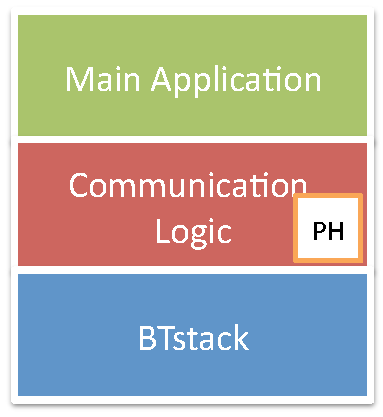
\includegraphics[width=0.3\textwidth]{picts/singlethreading-btstack.pdf} 
   \caption{BTstack in single-threaded environment. }
   \label{fig:BTstackSingle}
\end{figure}

BTstack provides a basic run loop that supports the concept of data sources and timers, which can be registered centrally. This works well when working with a small MCU and without an operating system.
To adapt to a basic operating system or a different scheduler, BTstack's run loop can be implemented based on the functions and mechanism of the existing system. 

Currently, we have two examples for this:
\begin{itemize}
\item \emph{run\_loop\_cocoa.c} is an implementation for the CoreFoundation Framework used in OS X and iOS. All run loop functions are implemented in terms of CoreFoundation calls, data sources and timers are modeled as CFSockets and CFRunLoopTimer respectively. 
\item \emph{run\_loop\_posix.c} is an implementation for POSIX compliant systems. The data sources are modeled as file descriptors and managed in a linked list. Then, the\emph{select} function is used to wait for the next file descriptor to become ready or timer to expire. 
\end{itemize}

\subsection{Adapting BTstack for Multi-Threaded Environments}
\label{section:multithreading}

The basic execution model of BTstack is a general while loop. Aside from interrupt-driven UART and timers, everything happens in sequence. 
When using BTstack in a multi-threaded environment,  this assumption has to stay valid - at least with respect to BTstack. For this, there are two common options:

\begin{figure}[ht]
\begin{minipage}[b]{\linewidth}
\centering
   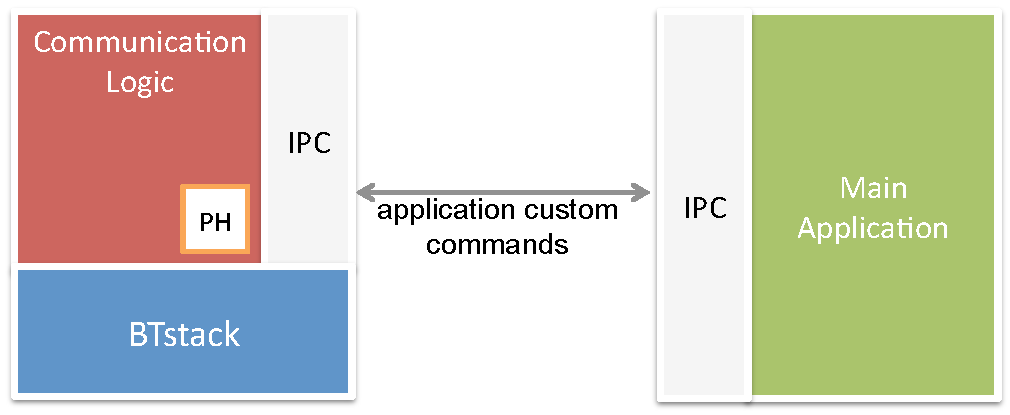
\includegraphics[width=0.8\textwidth]{picts/multithreading-monolithic.pdf} 
   \caption{BTstack in multi-threaded environment - monolithic solution.}
   \label{fig:BTstackMonolithic}
\vspace{0.8cm}
\end{minipage}

\begin{minipage}[b]{\linewidth}
\centering
   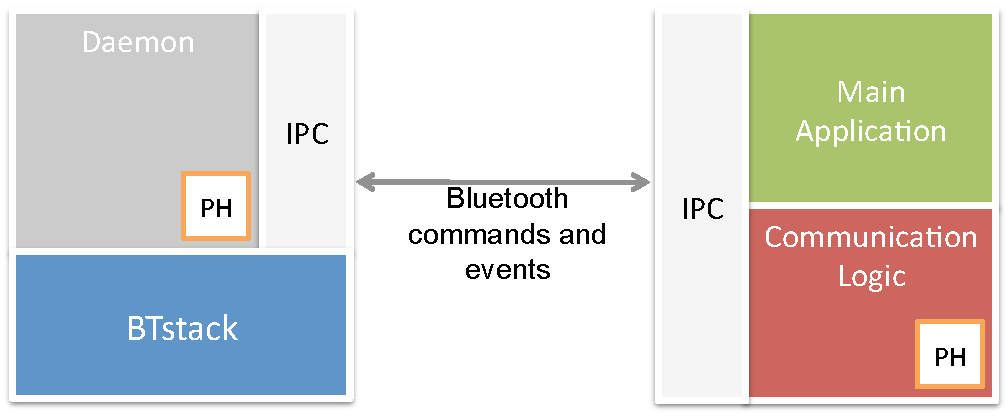
\includegraphics[width=0.8\textwidth]{picts/multithreading-btdaemon.pdf} 
   \caption{BTstack in multi-threaded environment - solution with daemon.}
   \label{fig:BTstackDaemon}
\end{minipage}
\end{figure}

\begin{itemize}
\item The Communication Logic is implemented on a dedicated BTstack thread, and the Main Application communicates with the BTstack thread via application-specific messages over an Interprocess Communication (IPC) as depicted in Figure \ref{fig:BTstackMonolithic}. This option results in less code and quick adaption.
\item BTstack must be extended to run standalone, i.e, as a Daemon, on a dedicated thread and the Main Application controls this daemon via BTstack extended HCI command over IPC - this is used for the non-embedded version of BTstack e.g., on the iPhone and it is depicted in Figure \ref{fig:BTstackDaemon}. This option requires more code but provides more flexibility.
\end{itemize}


\pagebreak

\appendix
	% !TEX root = btstack_gettingstarted.tex

% !TEX root = btstack_gettingstarted.tex
\section{Run Loop}
\label{appendix:api_run_loop}
$ $
\begin{lstlisting}
// Set timer based on current time in milliseconds.
void run_loop_set_timer(timer_source_t *a, uint32_t timeout_in_ms);

// Set callback that will be executed when timer expires.
void run_loop_set_timer_handler(timer_source_t *ts, void (*process)(timer_source_t *_ts));

// Add/Remove timer source.
void run_loop_add_timer(timer_source_t *timer); 
int  run_loop_remove_timer(timer_source_t *timer);

// Init must be called before any other run_loop call. 
// Use RUN_LOOP_EMBEDDED for embedded devices.
void run_loop_init(RUN_LOOP_TYPE type);

// Set data source callback.
void run_loop_set_data_source_handler(data_source_t *ds, int (*process)(data_source_t *_ds));

// Add/Remove data source.
void run_loop_add_data_source(data_source_t *dataSource);
int  run_loop_remove_data_source(data_source_t *dataSource);

// Execute configured run loop. This function does not return.
void run_loop_execute(void);

// hack to fix HCI timer handling
#ifdef HAVE_TICK
// Sets how many miliseconds has one tick.
uint32_t embedded_ticks_for_ms(uint32_t time_in_ms);
// Queries the current time in ticks.
uint32_t embedded_get_ticks(void);
// Queries the current time in ms
uint32_t embedded_get_time_ms(void);
// Allows to update BTstack system ticks based on another already 
// existing clock.
void embedded_set_ticks(uint32_t ticks);
#endif
#ifdef EMBEDDED
// Sets an internal flag that is checked in the critical section
// just before entering sleep mode. Has to be called by the interupt
// handler of a data source to signal the run loop that a new data 
// is available.
void embedded_trigger(void);    
// Execute run_loop once. It can be used to integrate BTstack's 
// timer and data source processing into a foreign run runloop 
// (it is not recommended).
void embedded_execute_once(void);
#endif
\end{lstlisting}
\pagebreak

% !TEX root = btstack_gettingstarted.tex
\section{Host Controller Interface (HCI) API}
\label{appendix:api_hci}
$ $
\begin{lstlisting}
// Set up HCI.
void hci_init(hci_transport_t *transport, void *config, bt_control_t *control, remote_device_db_t const* remote_device_db);

// Used if L2CAP is not used (rarely). 
void hci_register_packet_handler(void (*handler)(uint8_t packet_type, uint8_t *packet, uint16_t size));

// Requests the change of BTstack power mode.
int  hci_power_control(HCI_POWER_MODE mode);

// Allows to control if device is dicoverable. OFF by default.
void hci_discoverable_control(uint8_t enable);

// Creates and sends HCI command packets based on a template and 
// a list of parameters. Will return error if outgoing data buffer 
// is occupied. 
int hci_send_cmd(const hci_cmd_t *cmd, ...);

// Deletes link key for remote device with baseband address.
void hci_drop_link_key_for_bd_addr(bd_addr_t *addr);
\end{lstlisting}
\pagebreak
% !TEX root = btstack_gettingstarted.tex
\section{L2CAP API}
\label{appendix:api_l2cap}
$ $
\begin{lstlisting}
// Set up L2CAP and register L2CAP with HCI layer.
void l2cap_init(void);

// Registers a packet handler that handles HCI and general BTstack
// events.
void l2cap_register_packet_handler(void (*handler)(void * connection, uint8_t packet_type, uint16_t channel, uint8_t *packet, uint16_t size));

// Creates L2CAP channel to the PSM of a remote device with baseband
// address. A new baseband connection will be initiated if needed.
void l2cap_create_channel_internal(void * connection, btstack_packet_handler_t packet_handler, bd_addr_t address, uint16_t psm, uint16_t mtu);

// Disconencts L2CAP channel with given identifier. 
void l2cap_disconnect_internal(uint16_t local_cid, uint8_t reason);

// Queries the maximal transfer unit (MTU) for L2CAP channel with
// given identifier. 
uint16_t l2cap_get_remote_mtu_for_local_cid(uint16_t local_cid);

// Sends L2CAP data packet to the channel with given identifier.
int l2cap_send_internal(uint16_t local_cid, uint8_t *data, uint16_t len);

// Registers L2CAP service with given PSM and MTU, and assigns a
// packet handler. On embedded systems, use NULL for connection
// parameter.
void l2cap_register_service_internal(void *connection, btstack_packet_handler_t packet_handler, uint16_t psm, uint16_t mtu);

// Unregisters L2CAP service with given PSM.  On embedded systems,
// use NULL for connection parameter.
void l2cap_unregister_service_internal(void *connection, uint16_t psm);

// Accepts/Deny incoming L2CAP connection.
void l2cap_accept_connection_internal(uint16_t local_cid);
void l2cap_decline_connection_internal(uint16_t local_cid, uint8_t reason);
\end{lstlisting}
\pagebreak
% !TEX root = btstack_gettingstarted.tex
\section{RFCOMM API}
\label{appendix:api_rfcomm}
$ $
\begin{lstlisting}
// Set up RFCOMM.
void rfcomm_init(void);

// Register packet handler.
void rfcomm_register_packet_handler(void (*handler)(void *connection, uint8_t packet_type, uint16_t channel, uint8_t *packet, uint16_t size));

// Creates RFCOMM connection (channel) to a given server channel on 
// a remote device with baseband address. A new baseband connection 
// will be initiated if necessary.
// This connection is an RFCOMM channel. The channel will 
// automatically provide enough credits to the remote side.
void rfcomm_create_channel_internal(void *connection, bd_addr_t *addr, uint8_t channel);

// Creates RFCOMM connection (channel) to a given server channel on
// a remote device with baseband address. A new baseband connection
// will be initiated if necessary. 
// This channel will use explicit credit management. During channel 
// establishment, an initial amount of credits is provided.
void rfcomm_create_channel_with_initial_credits_internal(void *connection, bd_addr_t *addr, uint8_t server_channel, uint8_t initial_credits);

// Disconencts RFCOMM channel with given identifier. 
void rfcomm_disconnect_internal(uint16_t rfcomm_cid);

// Registers RFCOMM service for a server channel and a maximum frame 
// size, and assigns a packet handler. On embedded systems, use NULL 
// for connection parameter. This channel will automatically provide 
// enough credits to the remote side.
void rfcomm_register_service_internal(void *connection, uint8_t channel, uint16_t max_frame_size);

// Registers RFCOMM service for a server channel and a maximum frame
// size, and assigns a packet handler. On embedded systems, use NULL 
// for connection parameter.  This channel will use explicit credit
// management. During channel establishment, an initial amount of 
// credits is provided.
void rfcomm_register_service_with_initial_credits_internal(void *connection, uint8_t channel, uint16_t max_frame_size, uint8_t initial_credits);

// Unregister RFCOMM service.
void rfcomm_unregister_service_internal(uint8_t service_channel);

// Accepts/Deny incoming RFCOMM connection.
void rfcomm_accept_connection_internal(uint16_t rfcomm_cid);
void rfcomm_decline_connection_internal(uint16_t rfcomm_cid);


// Grant more incoming credits to the remote side for the given 
// RFCOMM channel identifier.
void rfcomm_grant_credits(uint16_t rfcomm_cid, uint8_t credits);

// Sends RFCOMM data packet to the RFCOMM channel with given
// identifier.
int  rfcomm_send_internal(uint16_t rfcomm_cid, uint8_t *data, uint16_t len); 
\end{lstlisting}
\pagebreak
% !TEX root = btstack_gettingstarted.tex
\section{SDP}
\label{appendix:api_sdp}
$ $
\begin{lstlisting}
// Set up SDP.
void sdp_init(void);

void sdp_register_packet_handler(void (*handler)(void * connection, uint8_t packet_type, uint16_t channel, uint8_t *packet, uint16_t size));

#ifdef EMBEDDED
// Register service record internally - this version doesn't copy 
// the record therefore it must be forever accessible.
// Preconditions:
//     - AttributeIDs are in ascending order;
//     - ServiceRecordHandle is first attribute and valid.
// @returns ServiceRecordHandle or 0 if registration failed.
uint32_t sdp_register_service_internal(void *connection, service_record_item_t * record_item);
#endif

#ifndef EMBEDDED
// Register service record internally - this version creates a copy
// of the record precondition: AttributeIDs are in ascending order
// => ServiceRecordHandle is first attribute if present.
// @returns ServiceRecordHandle or 0 if registration failed
uint32_t sdp_register_service_internal(void *connection, uint8_t * service_record);
#endif

// Unregister service record internally.
void sdp_unregister_service_internal(void *connection, uint32_t service_record_handle);
\end{lstlisting}
\pagebreak

% !TEX root = btstack_gettingstarted.tex
\section{SDP Client API}
\label{appendix:api_sdp_client}
$ $
\begin{lstlisting}
 
/** 
 * @brief Queries the SDP service of the remote device given a service search pattern and a list of attribute IDs. The remote data is handled by the SDP parser. The SDP parser delivers attribute values and done event via a registered callback.
 */
void sdp_client_query(bd_addr_t remote, uint8_t * des_serviceSearchPattern, uint8_t * des_attributeIDList);

#ifdef HAVE_SDP_EXTRA_QUERIES
void sdp_client_service_attribute_search(bd_addr_t remote, uint32_t search_serviceRecordHandle, uint8_t * des_attributeIDList);
void sdp_client_service_search(bd_addr_t remote, uint8_t * des_serviceSearchPattern);
#endif
\end{lstlisting}
\pagebreak

% !TEX root = btstack_gettingstarted.tex
\section{SDP Query API}
\label{appendix:api_sdp_query}
$ $
 \begin{lstlisting}
/* SDP Queries */

// Basic SDP Query event type.
typedef struct sdp_query_event {
    uint8_t type;
} sdp_query_event_t;

// SDP Query event to indicate that query is complete.
typedef struct sdp_query_complete_event {
    uint8_t type;
    uint8_t status; // 0 == OK
} sdp_query_complete_event_t;



/* SDP Query for RFCOMM */

// SDP Query RFCOMM event to deliver channel number and service 
// name byte by byte.
typedef struct sdp_query_rfcomm_service_event {
    uint8_t type;
    uint8_t channel_nr;
    uint8_t * service_name;
} sdp_query_rfcomm_service_event_t;

// Searches SDP records on a remote device for RFCOMM services with
// a given UUID.
void sdp_query_rfcomm_channel_and_name_for_uuid(bd_addr_t remote, uint16_t uuid);

// Searches SDP records on a remote device for RFCOMM services with 
// a given service search pattern.
void sdp_query_rfcomm_channel_and_name_for_search_pattern(bd_addr_t remote, uint8_t * des_serviceSearchPattern);

// Registers a callback to receive RFCOMM service and query complete
// event. 
void sdp_query_rfcomm_register_callback(void(*sdp_app_callback)(sdp_query_event_t * event, void * context), void * context);
\end{lstlisting}
\pagebreak
% !TEX root = btstack_gettingstarted.tex
\section{GATT Client API}
\label{appendix:api_gatt_client}
$ $
\begin{lstlisting}
// Set up GATT client.
void gatt_client_init();

// Register callback (packet handler) for gatt client. Returns gatt client ID.
uint16_t gatt_client_register_packet_handler (gatt_client_callback_t callback);

// Unregister callback (packet handler) for gatt client.
void gatt_client_unregister_packet_handler(uint16_t gatt_client_id);

// Returns the GATT client context for the specified handle.
// gatt_client_t * get_gatt_client_context_for_handle(uint16_t con_handle);

// Returns if the gatt client is ready to receive a query. It is used with daemon.
int gatt_client_is_ready(uint16_t handle);

// Discovers all primary services. For each found service, an
// le_service_event_t with type set to GATT_SERVICE_QUERY_RESULT
// will be generated and passed to the registered callback.
// The gatt_complete_event_t, with type set to GATT_QUERY_COMPLETE,
// marks the end of discovery.
le_command_status_t gatt_client_discover_primary_services(uint16_t gatt_client_id, uint16_t con_handle);

// Discovers a specific primary service given its UUID. This service
// may exist multiple times. For each found service, an
// le_service_event_t with type set to GATT_SERVICE_QUERY_RESULT
// will be generated and passed to the registered callback.
// The gatt_complete_event_t, with type set to GATT_QUERY_COMPLETE,
// marks the end of discovery.
le_command_status_t gatt_client_discover_primary_services_by_uuid16(uint16_t gatt_client_id, uint16_t con_handle, uint16_t uuid16);
le_command_status_t gatt_client_discover_primary_services_by_uuid128(uint16_t gatt_client_id, uint16_t con_handle, const uint8_t * uuid);

// Finds included services within the specified service. For each
// found included service, an le_service_event_t with type set to
// GATT_INCLUDED_SERVICE_QUERY_RESULT will be generated and passed
// to the registered callback. The gatt_complete_event_t with type
// set to GATT_QUERY_COMPLETE, marks the end of discovery.
//
// Information about included service type (primary/secondary) can
// be retrieved either by sending an ATT find information request
// for the returned start group handle (returning the handle and
// the UUID for primary or secondary service) or by comparing the
// service to the list of all primary services.
le_command_status_t gatt_client_find_included_services_for_service(uint16_t gatt_client_id, uint16_t con_handle, le_service_t *service);

// Discovers all characteristics within the specified service. For
// each found characteristic, an le_characteristics_event_t with 
// type set to GATT_CHARACTERISTIC_QUERY_RESULT will be generated 
// and passed to the registered callback. The gatt_complete_event_t 
// with type set to GATT_QUERY_COMPLETE, marks the end of discovery.
le_command_status_t gatt_client_discover_characteristics_for_service(uint16_t gatt_client_id, uint16_t con_handle, le_service_t *service);

// The following four functions are used to discover all 
// characteristics within the specified service or handle range, and 
// return those that match the given UUID. For each found
// characteristic, an le_characteristic_event_t with type set to   
// GATT_CHARACTERISTIC_QUERY_RESULT will be generated and passed to 
// the registered callback. The gatt_complete_event_t with type set
// to GATT_QUERY_COMPLETE, marks the end of discovery.
le_command_status_t gatt_client_discover_characteristics_for_handle_range_by_uuid16(uint16_t gatt_client_id, uint16_t con_handle, uint16_t start_handle, uint16_t end_handle, uint16_t uuid16);
le_command_status_t gatt_client_discover_characteristics_for_handle_range_by_uuid128(uint16_t gatt_client_id, uint16_t con_handle, uint16_t start_handle, uint16_t end_handle, uint8_t * uuid);
le_command_status_t gatt_client_discover_characteristics_for_service_by_uuid16 (uint16_t gatt_client_id, uint16_t con_handle, le_service_t *service, uint16_t  uuid16);
le_command_status_t gatt_client_discover_characteristics_for_service_by_uuid128(uint16_t gatt_client_id, uint16_t con_handle, le_service_t *service, uint8_t * uuid128);

// Discovers attribute handle and UUID of a characteristic 
// descriptor within the specified characteristic. For each found
// descriptor, an le_characteristic_descriptor_event_t with 
// type set to GATT_CHARACTERISTIC_DESCRIPTOR_QUERY_RESULT will be  
// generated and passed to the registered callback. The  
// gatt_complete_event_t with type set to GATT_QUERY_COMPLETE, marks 
// the end of discovery.
le_command_status_t gatt_client_discover_characteristic_descriptors(uint16_t gatt_client_id, uint16_t con_handle, le_characteristic_t *characteristic);

// Reads the characteristic value using the characteristic's value
// handle. If the characteristic value is found, an 
// le_characteristic_value_event_t with type set to 
// GATT_CHARACTERISTIC_VALUE_QUERY_RESULT will be generated and
// passed to the registered callback. The gatt_complete_event_t 
// with type set to GATT_QUERY_COMPLETE, marks the end of read.
le_command_status_t gatt_client_read_value_of_characteristic(uint16_t gatt_client_id, uint16_t con_handle, le_characteristic_t *characteristic);
le_command_status_t gatt_client_read_value_of_characteristic_using_value_handle(uint16_t gatt_client_id, uint16_t con_handle, uint16_t characteristic_value_handle);

// Reads the long characteristic value using the characteristic's 
// value handle. The value will be returned in several blobs. For 
// each blob, an le_characteristic_value_event_t with type set to 
// GATT_CHARACTERISTIC_VALUE_QUERY_RESULT and updated value offset
// will be generated and passed to the registered callback. The 
// gatt_complete_event_t with type set to GATT_QUERY_COMPLETE, marks
// the end of read.
le_command_status_t gatt_client_read_long_value_of_characteristic(uint16_t gatt_client_id, uint16_t con_handle, le_characteristic_t *characteristic);
le_command_status_t gatt_client_read_long_value_of_characteristic_using_value_handle(uint16_t gatt_client_id, uint16_t con_handle, uint16_t characteristic_value_handle);
    
// Writes the characteristic value using the characteristic's value
// handle without an acknowledgement that the write was successfully
// performed.
le_command_status_t gatt_client_write_value_of_characteristic_without_response(uint16_t gatt_client_id, uint16_t con_handle, uint16_t characteristic_value_handle, uint16_t length, uint8_t * data);

// Writes the authenticated characteristic value using the
// characteristic's value handle without an acknowledgement
// that the write was successfully performed.
le_command_status_t gatt_client_signed_write_without_response(uint16_t gatt_client_id, uint16_t con_handle, uint16_t handle, uint16_t message_len, uint8_t * message, sm_key_t csrk, uint32_t sgn_counter);

// Writes the characteristic value using the characteristic's value
// handle. The gatt_complete_event_t with type set to
// GATT_QUERY_COMPLETE, marks the end of write. The write is
// successfully performed, if the event's status field is set to 0.
le_command_status_t gatt_client_write_value_of_characteristic(uint16_t gatt_client_id, uint16_t con_handle, uint16_t characteristic_value_handle, uint16_t length, uint8_t * data);
le_command_status_t gatt_client_write_long_value_of_characteristic(uint16_t gatt_client_id, uint16_t con_handle, uint16_t characteristic_value_handle, uint16_t length, uint8_t * data);

// Writes of the long characteristic value using the
// characteristic's value handle. It uses server response to
// validate that the write was correctly received.
// The gatt_complete_event_t with type set to GATT_QUERY_COMPLETE
// marks the end of write. The write is successfully performed, if
// the event's status field is set to 0.
le_command_status_t gatt_client_reliable_write_long_value_of_characteristic(uint16_t gatt_client_id, uint16_t con_handle, uint16_t characteristic_value_handle, uint16_t length, uint8_t * data);

// Reads the characteristic descriptor using its handle. If the
// characteristic descriptor is found, an
// le_characteristic_descriptor_event_t with type set to
// GATT_CHARACTERISTIC_DESCRIPTOR_QUERY_RESULT will be generated
// and passed to the registered callback. The gatt_complete_event_t
// with type set to GATT_QUERY_COMPLETE, marks the end of read.
le_command_status_t gatt_client_read_characteristic_descriptor(uint16_t gatt_client_id, uint16_t con_handle, le_characteristic_descriptor_t * descriptor);

// Reads the long characteristic descriptor using its handle. It
// will be returned in several blobs.  For each blob, an
// le_characteristic_descriptor_event_t with type set to
// GATT_CHARACTERISTIC_DESCRIPTOR_QUERY_RESULT will be generated
// and passed to the registered callback. The gatt_complete_event_t
// with type set to GATT_QUERY_COMPLETE, marks the end of read.
le_command_status_t gatt_client_read_long_characteristic_descriptor(uint16_t gatt_client_id, uint16_t con_handle, le_characteristic_descriptor_t * descriptor);

// Writes the characteristic descriptor using its handle.
// The gatt_complete_event_t with type set to
// GATT_QUERY_COMPLETE, marks the end of write. The write is
// successfully performed, if the event's status field is set to 0.
le_command_status_t gatt_client_write_characteristic_descriptor(uint16_t gatt_client_id, uint16_t con_handle, le_characteristic_descriptor_t * descriptor, uint16_t length, uint8_t * data);
le_command_status_t gatt_client_write_long_characteristic_descriptor(uint16_t gatt_client_id, uint16_t con_handle, le_characteristic_descriptor_t * descriptor, uint16_t length, uint8_t * data);

// Writes the client characteristic configuration of the specified 
// characteristic. It is used to subscribe for notifications or 
// indications of the characteristic value. For notifications or 
// indications specify:
// GATT_CLIENT_CHARACTERISTICS_CONFIGURATION_NOTIFICATION resp. 
// GATT_CLIENT_CHARACTERISTICS_CONFIGURATION_INDICATION 
// as configuration value.
le_command_status_t gatt_client_write_client_characteristic_configuration(uint16_t gatt_client_id, uint16_t con_handle, le_characteristic_t * characteristic, uint16_t configuration);
\end{lstlisting}
\pagebreak
% !TEX root = btstack_gettingstarted.tex
\section{PAN API}
\label{appendix:api_pan}
$ $
\begin{lstlisting}
/** 
 * @brief Creates SDP record for PANU BNEP service in provided empty buffer.
 * @note Make sure the buffer is big enough.
 *
 * @param service is an empty buffer to store service record
 * @param security_desc 
 * @param name if NULL, the default service name will be assigned
 * @param description if NULL, the default service description will be assigned
 */
void pan_create_panu_service(uint8_t *service, const char *name, const char *description, security_description_t security_desc);

/** 
 * @brief Creates SDP record for GN BNEP service in provided empty buffer.
 * @note Make sure the buffer is big enough.
 *
 * @param service is an empty buffer to store service record
 * @param security_desc 
 * @param name if NULL, the default service name will be assigned
 * @param description if NULL, the default service description will be assigned
 * @param IPv4Subnet is optional subnet definition, e.g. "10.0.0.0/8"
 * @param IPv6Subnet is optional subnet definition given in the standard IETF format with the absolute attribute IDs
 */
void pan_create_gn_service(uint8_t *service, const char *name, const char *description, security_description_t security_desc, 
	const char *IPv4Subnet, const char *IPv6Subnet);

/** 
 * @brief Creates SDP record for NAP BNEP service in provided empty buffer.
 * @note Make sure the buffer is big enough.
 *
 * @param service is an empty buffer to store service record
 * @param name if NULL, the default service name will be assigned
 * @param security_desc 
 * @param description if NULL, the default service description will be assigned
 * @param net_access_type type of available network access
 * @param max_net_access_rate based on net_access_type measured in byte/s
 * @param IPv4Subnet is optional subnet definition, e.g. "10.0.0.0/8"
 * @param IPv6Subnet is optional subnet definition given in the standard IETF format with the absolute attribute IDs
 */
void pan_create_nap_service(uint8_t *service, const char *name, const char *description, security_description_t security_desc, 
	net_access_type_t net_access_type, uint32_t max_net_access_rate, const char *IPv4Subnet, const char *IPv6Subnet);
\end{lstlisting}
\pagebreak

% !TEX root = btstack_gettingstarted.tex
\section{BNEP API}
\label{appendix:api_bnep}
$ $
\begin{lstlisting}
/**
 * @brief Set up BNEP.
 */
void bnep_init(void);

/**
 * @brief Check if a data packet can be send out.
 */
int bnep_can_send_packet_now(uint16_t bnep_cid);

/**
 * @brief Send a data packet.
 */
int bnep_send(uint16_t bnep_cid, uint8_t *packet, uint16_t len);

/**
 * @brief Set the network protocol filter.
 */
int bnep_set_net_type_filter(uint16_t bnep_cid, bnep_net_filter_t *filter, uint16_t len);

/**
 * @brief Set the multicast address filter.
 */
int bnep_set_multicast_filter(uint16_t bnep_cid, bnep_multi_filter_t *filter, uint16_t len);

/**
 * @brief Set security level required for incoming connections, need to be called before registering services.
 */
void bnep_set_required_security_level(gap_security_level_t security_level);

/**
 * @brief Register packet handler. 
 */
void bnep_register_packet_handler(void (*handler)(void * connection, uint8_t packet_type, uint16_t channel, uint8_t *packet, uint16_t size));

/**
 * @brief Creates BNEP connection (channel) to a given server on a remote device with baseband address. A new baseband connection will be initiated if necessary. 
 */
int bnep_connect(void * connection, bd_addr_t addr, uint16_t l2cap_psm, uint16_t uuid_dest);

/**
 * @brief Disconnects BNEP channel with given identifier. 
 */
void bnep_disconnect(bd_addr_t addr);

/**
 * @brief Registers BNEP service, set a maximum frame size and assigns a packet handler. On embedded systems, use NULL for connection parameter. 
 */
void bnep_register_service(void * connection, uint16_t service_uuid, uint16_t max_frame_size);

/**
 * @brief Unregister BNEP service.
 */
void bnep_unregister_service(uint16_t service_uuid);
\end{lstlisting}
\pagebreak

% !TEX root = btstack_gettingstarted.tex
\section{GAP API}
\label{appendix:api_gap}
$ $
\begin{lstlisting}
/**
 * @brief Enable/disable bonding. Default is enabled.
 * @param enabled
 */
void gap_set_bondable_mode(int enabled);

/**
 * @brief Start dedicated bonding with device. Disconnect after bonding.
 * @param device
 * @param request MITM protection
 * @return error, if max num acl connections active
 * @result GAP_DEDICATED_BONDING_COMPLETE
 */
int gap_dedicated_bonding(bd_addr_t device, int mitm_protection_required);

gap_security_level_t gap_security_level_for_link_key_type(link_key_type_t link_key_type);
gap_security_level_t gap_security_level(hci_con_handle_t con_handle);

void gap_request_security_level(hci_con_handle_t con_handle, gap_security_level_t level);
int  gap_mitm_protection_required_for_security_level(gap_security_level_t level);

/** 
 * @brief Sets local name.
 * @note has to be done before stack starts up
 * @param name is not copied, make sure memory is accessible during stack startup
 */
void gap_set_local_name(const char * local_name);
\end{lstlisting}
\pagebreak

% !TEX root = btstack_gettingstarted.tex
\section{SM API}
\label{appendix:api_sm}
$ $
\begin{lstlisting}
/**
 * @brief Security Manager event
 */
typedef struct sm_event {
    uint8_t   type;                 ///< See <btstack/hci_cmds.h> SM_...
    uint8_t   addr_type;
    bd_addr_t address;
    uint32_t  passkey;              ///< only used for SM_PASSKEY_DISPLAY_NUMBER 
    uint16_t  le_device_db_index;   ///< only used for SM_IDENTITY_RESOLVING_..
    uint8_t   authorization_result; ///< only use for SM_AUTHORIZATION_RESULT
} sm_event_t;

/**
 * @brief Initializes the Security Manager, connects to L2CAP
 */
void sm_init();

/**
 * @brief Set secret ER key for key generation as described in Core V4.0, Vol 3, Part G, 5.2.2 
 * @param er
 */
void sm_set_er(sm_key_t er);

/**
 * @brief Set secret IR key for key generation as described in Core V4.0, Vol 3, Part G, 5.2.2 
 */
void sm_set_ir(sm_key_t ir);

/**
 *
 * @brief Registers OOB Data Callback. The callback should set the oob_data and return 1 if OOB data is availble
 * @param get_oob_data_callback
 */
void sm_register_oob_data_callback( int (*get_oob_data_callback)(uint8_t addres_type, bd_addr_t addr, uint8_t * oob_data));

/**
 *
 * @brief Registers packet handler. Called by att_server.c
 */
void sm_register_packet_handler(btstack_packet_handler_t handler);

/**
 * @brief Limit the STK generation methods. Bonding is stopped if the resulting one isn't in the list
 * @param OR combination of SM_STK_GENERATION_METHOD_ 
 */
void sm_set_accepted_stk_generation_methods(uint8_t accepted_stk_generation_methods);

/**
 * @brief Set the accepted encryption key size range. Bonding is stopped if the result isn't within the range
 * @param min_size (default 7)
 * @param max_size (default 16)
 */
void sm_set_encryption_key_size_range(uint8_t min_size, uint8_t max_size);

/**
 * @brief Sets the requested authentication requirements, bonding yes/no, MITM yes/no
 * @param OR combination of SM_AUTHREQ_ flags
 */
void sm_set_authentication_requirements(uint8_t auth_req);

/**
 * @brief Sets the available IO Capabilities
 * @param IO_CAPABILITY_
 */
void sm_set_io_capabilities(io_capability_t io_capability);

/**
 * @brief Let Peripheral request an encrypted connection right after connecting
 * @note Not used normally. Bonding is triggered by access to protected attributes in ATT Server
 */
void sm_set_request_security(int enable);

/** 
 * @brief Trigger Security Request
 * @note Not used normally. Bonding is triggered by access to protected attributes in ATT Server
 */
void sm_send_security_request(uint16_t handle);

/**
 * @brief Decline bonding triggered by event before
 * @param addr_type and address
 */
void sm_bonding_decline(uint8_t addr_type, bd_addr_t address);

/**
 * @brief Confirm Just Works bonding 
 * @param addr_type and address
 */
void sm_just_works_confirm(uint8_t addr_type, bd_addr_t address);

/**
 * @brief Reports passkey input by user
 * @param addr_type and address
 * @param passkey in [0..999999]
 */
void sm_passkey_input(uint8_t addr_type, bd_addr_t address, uint32_t passkey);

/**
 *
 * @brief Get encryption key size.
 * @param addr_type and address
 * @return 0 if not encrypted, 7-16 otherwise
 */
int sm_encryption_key_size(uint8_t addr_type, bd_addr_t address);

/**
 * @brief Get authentication property.
 * @param addr_type and address
 * @return 1 if bonded with OOB/Passkey (AND MITM protection)
 */
int sm_authenticated(uint8_t addr_type, bd_addr_t address);

/**
 * @brief Queries authorization state.
 * @param addr_type and address
 * @return authorization_state for the current session
 */
authorization_state_t sm_authorization_state(uint8_t addr_type, bd_addr_t address);

/**
 * @brief Used by att_server.c to request user authorization.
 * @param addr_type and address
 */
void sm_request_authorization(uint8_t addr_type, bd_addr_t address);

/**
 * @brief Report user authorization decline.
 * @param addr_type and address
 */
void sm_authorization_decline(uint8_t addr_type, bd_addr_t address);

/**
 * @brief Report user authorization grant.
 * @param addr_type and address
 */
void sm_authorization_grant(uint8_t addr_type, bd_addr_t address);

/**
 * @brief Support for signed writes, used by att_server.
 * @note Message and result are in little endian to allows passing in ATT PDU without flipping them first.
 */
int  sm_cmac_ready();
void sm_cmac_start(sm_key_t k, uint16_t message_len, uint8_t * message, uint32_t sign_counter, void (*done_handler)(uint8_t hash[8]));

/**
 * @brief Identify device in LE Device DB.
 * @param handle
 * @return index from le_device_db or -1 if not found/identified
 */
int sm_le_device_index(uint16_t handle );
\end{lstlisting}
\pagebreak

    
	% !TEX root = btstack_gettingstarted.tex
\section{Events and Errors}
\label{appendix:api_events_and_errors}

L2CAP events and data packets are delivered to the packet handler specified by \emph{l2cap\_register\_service} resp. \emph{l2cap\_create\_channel\_internal}. Data packets have the L2CAP\_DATA\_PACKET packet type. L2CAP provides the following events:
\begin{itemize}
\item L2CAP\_EVENT\_CHANNEL\_OPENED - sent if channel establishment is done. Status not equal zero indicates an error. Possible errors: out of memory; connection terminated by local host, when the connection to remote device fails.
\item L2CAP\_EVENT\_CHANNEL\_CLOSED - emitted when channel is closed. No status information is provided.
\item L2CAP\_EVENT\_INCOMING\_CONNECTION - received when the connection is requested  by remote. Connection accept and decline are performed with \emph{l2cap\_accept\_connection\_internal} and \emph{l2cap\_decline\_connecti-on\_internal} respectively.
\item L2CAP\_EVENT\_CREDITS - emitted when there is a chance to send a new L2CAP packet. BTstack does not buffer packets. Instead, it requires the application to retry sending if BTstack cannot deliver a packet to the Bluetooth module. In this case, the l2cap\_send\_internal will return an error. 
\item L2CAP\_EVENT\_SERVICE\_REGISTERED - Status not equal zero indicates an error. Possible errors: service is already registered; MAX\_NO-\_L2CAP\_SERVICES (defined in config.h) already registered.
\end{itemize}
 
\begin{table*}[bp]
\caption{L2CAP Events}
\begin{tabular}{p{1cm}p{10cm}c}\toprule
\multicolumn{2}{c}{Event / Event Parameters (size in bits) } & Event Code\\ 
\midrule
\multicolumn{2}{l}{L2CAP\_EVENT\_CHANNEL\_OPENED} & 0x70\\
&\emph{event(8), len(8), status(8), address(48), handle(16)}\\
&\emph{psm(16), local\_cid(16), remote\_cid(16), local\_mtu(16), }\\
&\emph{remote\_mtu(16)}\\
\\
\multicolumn{2}{l}{L2CAP\_EVENT\_CHANNEL\_CLOSED} & 0x71\\
&\emph{event (8), len(8), channel(16)}\\
\\
\multicolumn{2}{l}{L2CAP\_EVENT\_INCOMING\_CONNECTION}& 0x72\\
&\emph{event(8), len(8), address(48), handle(16), psm (16), }\\
&\emph{local\_cid(16), remote\_cid (16)}\\
\\
\multicolumn{2}{l}{L2CAP\_EVENT\_CREDITS} & 0x74\\
&\emph{event(8), len(8), local\_cid(16), credits(8)}\\
\\
\multicolumn{2}{l}{L2CAP\_EVENT\_SERVICE\_REGISTERED} & 0x75\\
&\emph{event(8), len(8), status(8), psm(16)}\\
\\
\bottomrule
 \label{table:l2capEvents}
\end{tabular}
\end{table*}

\pagebreak

All RFCOMM events and data packets are currently delivered to the packet handler specified by \emph{rfcomm\_register\_packet\_handler}. Data packets have the \mbox{RFCOMM}\_DATA\_PACKET packet type. Here is the list of events provided by RFCOMM:
\begin{itemize}
\item RFCOMM\_EVENT\_INCOMING\_CONNECTION - received when the connection is requested by remote. Connection accept and decline are performed with \emph{rfcomm\_accept\_connection\_internal} and \emph{rfcomm\_decline\_con-nection\_internal} respectively.
\item RFCOMM\_EVENT\_CHANNEL\_CLOSED - emitted when channel is closed. No status information is provided.
\item RFCOMM\_EVENT\_OPEN\_CHANNEL\_COMPLETE - sent if channel establishment is done. Status not equal zero indicates an error. Possible errors: an L2CAP error, out of memory.
\item RFCOMM\_EVENT\_CREDITS - The application can resume sending when this even is received. See Section \ref{section:flowcontrol} for more on RFCOMM credit-based flow-control.
\item RFCOMM\_EVENT\_SERVICE\_REGISTERED - Status not equal zero indicates an error. Possible errors: service is already registered; MAX-\_NO\_RFCOMM\_SERVICES (defined in config.h) already registered.
\end{itemize}

\begin{table*}[bp]
\caption{RFCOMM Events}
\begin{tabular}{p{1cm}p{10cm}c}\toprule
\multicolumn{2}{c}{Event / Event Parameters (size in bits)} & Event Code\\ 
\midrule

\multicolumn{2}{l}{RFCOMM\_EVENT\_OPEN\_CHANNEL\_COMPLETE} & 0x80\\
&\emph{event(8), len(8), status(8), address(48), handle(16), }\\
&\emph{server\_channel(8), rfcomm\_cid(16), max\_frame\_size(16)}\\
\\
\multicolumn{2}{l}{RFCOMM\_EVENT\_CHANNEL\_CLOSED} & 0x81\\
&\emph{event(8), len(8), rfcomm\_cid(16)}\\
\\
\multicolumn{2}{l}{RFCOMM\_EVENT\_INCOMING\_CONNECTION}& 0x82\\
&\emph{event(8), len(8), address(48), channel (8),} \\
& \emph{rfcomm\_cid(16)}\\
\\
\multicolumn{2}{l}{RFCOMM\_EVENT\_CREDITS} & 0x84\\
&\emph{event(8), len(8), rfcomm\_cid(16), credits(8)}\\
\\
\multicolumn{2}{l}{RFCOMM\_EVENT\_SERVICE\_REGISTERED} & 0x85\\
&\emph{event(8), len(8), status(8), rfcomm server channel\_id(8)}\\
\bottomrule
 \label{table:rfcommEvents}
\end{tabular}
\end{table*}


\begin{table}
\caption{Errors}
\begin{tabular}{lc}\toprule
Error & Error Code\\ 
\midrule
{\tiny BTSTACK\_MEMORY\_ALLOC\_FAILED} & {\tiny 0x56}\\
{\tiny BTSTACK\_ACL\_BUFFERS\_FULL} & {\tiny 0x57}\\
{\tiny L2CAP\_COMMAND\_REJECT\_REASON\_COMMAND\_NOT\_UNDERSTOOD} & {\tiny 0x60}\\
{\tiny L2CAP\_COMMAND\_REJECT\_REASON\_SIGNALING\_MTU\_EXCEEDED} & {\tiny 0x61}\\
{\tiny L2CAP\_COMMAND\_REJECT\_REASON\_INVALID\_CID\_IN\_REQUEST} & {\tiny 0x62}\\
{\tiny L2CAP\_CONNECTION\_RESPONSE\_RESULT\_SUCCESSFUL} & {\tiny 0x63}\\
{\tiny L2CAP\_CONNECTION\_RESPONSE\_RESULT\_PENDING} & {\tiny 0x64}\\
{\tiny L2CAP\_CONNECTION\_RESPONSE\_RESULT\_REFUSED\_PSM} & {\tiny 0x65}\\
{\tiny L2CAP\_CONNECTION\_RESPONSE\_RESULT\_REFUSED\_SECURITY} & {\tiny 0x66}\\
{\tiny L2CAP\_CONNECTION\_RESPONSE\_RESULT\_REFUSED\_RESOURCES} & {\tiny 0x65}\\
{\tiny L2CAP\_CONFIG\_RESPONSE\_RESULT\_SUCCESSFUL} & {\tiny 0x66}\\
{\tiny L2CAP\_CONFIG\_RESPONSE\_RESULT\_UNACCEPTABLE\_PARAMS} & {\tiny 0x67}\\
{\tiny L2CAP\_CONFIG\_RESPONSE\_RESULT\_REJECTED} & {\tiny 0x68}\\
{\tiny L2CAP\_CONFIG\_RESPONSE\_RESULT\_UNKNOWN\_OPTIONS} & {\tiny 0x69}\\
{\tiny L2CAP\_SERVICE\_ALREADY\_REGISTERED} & {\tiny 0x6a}\\
{\tiny RFCOMM\_MULTIPLEXER\_STOPPED} & {\tiny 0x70}\\
{\tiny RFCOMM\_CHANNEL\_ALREADY\_REGISTERED} & {\tiny 0x71}\\
{\tiny RFCOMM\_NO\_OUTGOING\_CREDITS} & {\tiny 0x72}\\
{\tiny SDP\_HANDLE\_ALREADY\_REGISTERED} & {\tiny 0x80}\\
\bottomrule
\label{table:sdpErrors}
\end{tabular}
\end{table}

\begin{minipage}[t][5cm][t]{\textwidth}
\end{minipage}
\pagebreak

\pagebreak

\section{Revision History}
\label{appendix:revision_history}

\begin{table}[!htbp]
\begin{tabular*}{\textwidth}{lp{3.5cm}p{8.5cm}}\toprule
Rev & Date & Comments\\ 
\midrule
1.3 & November 6, 2014 & Introducing GATT client and server. Work in progress.\\
1.2 & November 1, 2013 & Explained Secure Simple Pairing in "Pairing of devices".\\
1.1 & August 30, 2013 & Introduced SDP client. Updated Quick Recipe on "Query remote SDP service".\\
\bottomrule
\end{tabular*}
\end{table}

%\section {TODO}
%
%\section {Maybe Missing}
%\begin{itemize}
%\item profiles in BTstack (SPP)
%\item More examples: HID mouse host, HID mouse device, HID keyboard device, BLE Client, ..
%\end{itemize}
%


% \bibliographystyle{IEEEtran}
% \bibliography{btstack-manual}

% \section*{Bibliography}

%\textbf{P. W. Wachulak} received the degree${\ldots}$ \\[6pt]
%\textbf{M. C. Marconi} received the degree${\ldots}$ \\[6pt]
%\textbf{R. A. Bartels} received the degree${\ldots}$ \\[6pt]
%\textbf{C. S. Menoni} received the degree${\ldots}$ \\[6pt]
%\textbf{J. J. Rocca} received the degree${\ldots}$


\end{document}